\section{1174043 Irvan Rizkiansyah}

	\subsection{Teori}
	\begin{enumerate}
		\item Jelaskan Apa Itu binari calssification dilengkapi ilustrasi gambar sendiri.\par
		Binary Classification merupakan kegiatan yang berguna untuk mengklasifikasikan elemen-elemen dari sebuah himpunan tertentu ke dalam dua kelompok berbeda (memprediksi kelompok mana yang masing-masing dimiliki) berdasarkan dari aturan klasifikasi.
		\begin{figure}[ht]
			\centering
			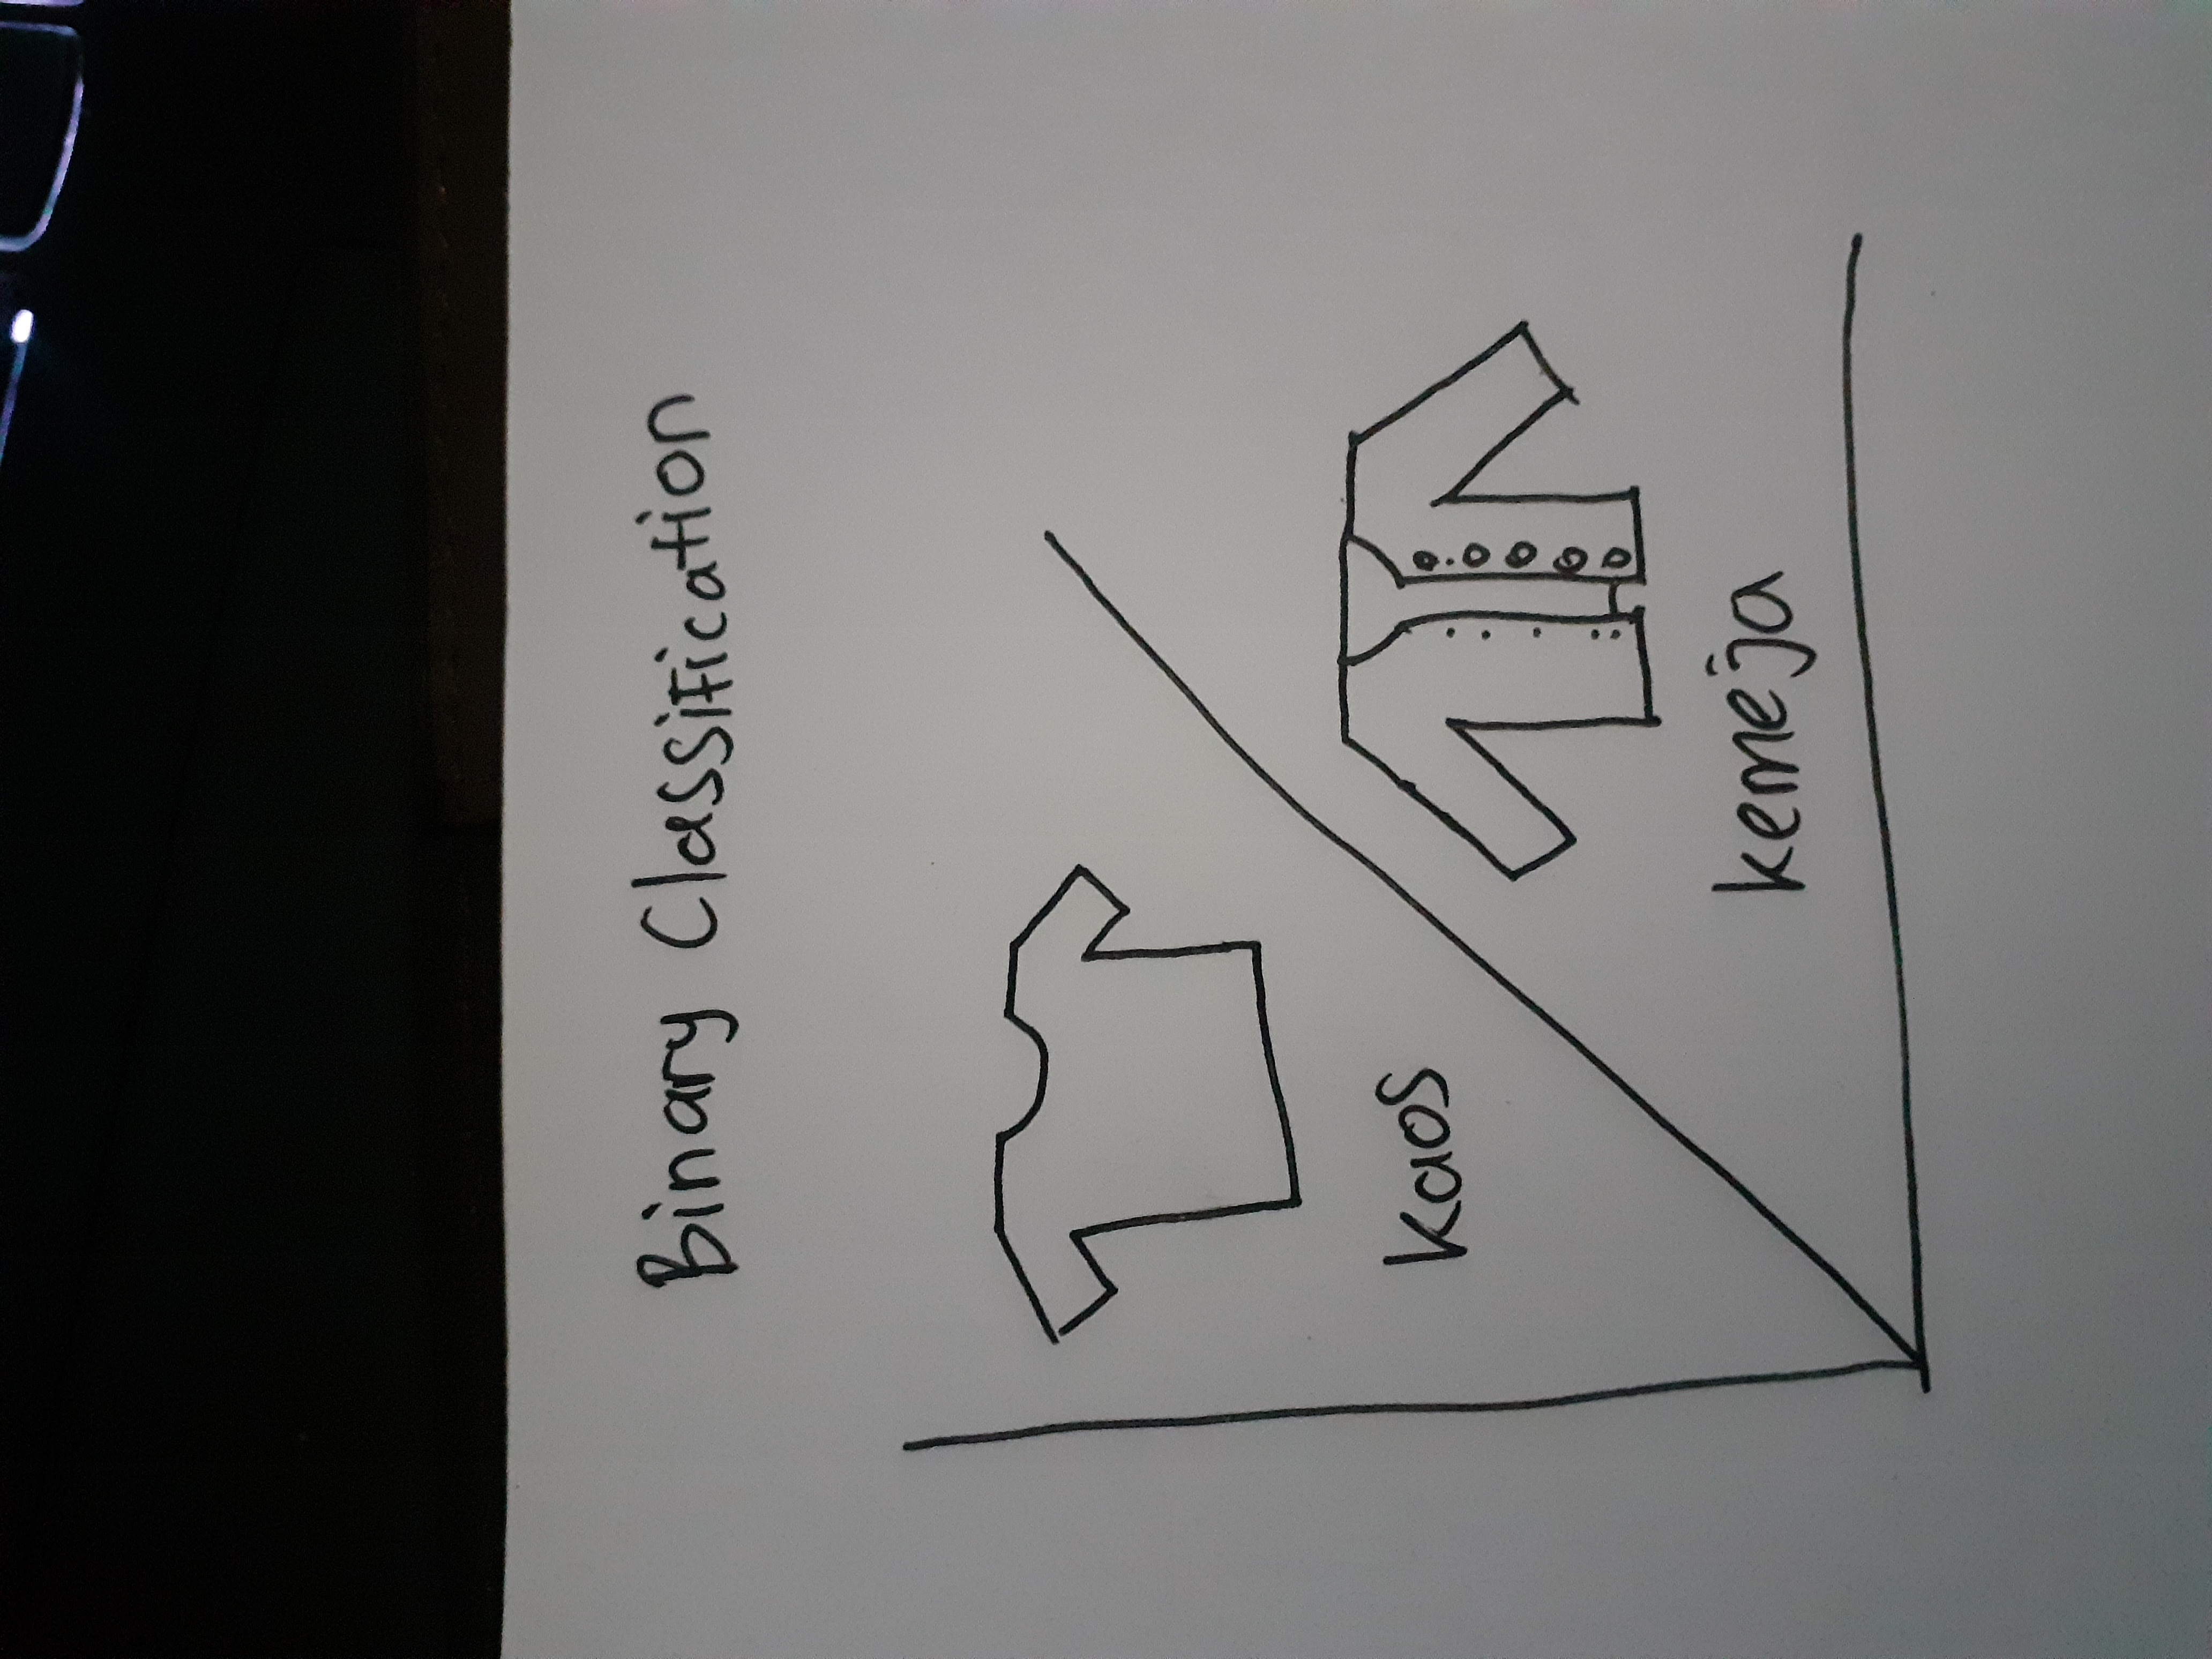
\includegraphics[scale=0.01]{figures/1174043/chapter2/1.jpg}
			\caption{contoh Binary Classification}
			\label{contoh}
		\end{figure}
		
		\item Jelaskan Apaitu supervised learning , unsupervised learning dan clusterring dengan ilustrasi gambar sendiri.\par
		Supervised learning adalah sebuah metode pendekatan yang mana sudah terdapat data yang dilatih, dan terdapat variabel yang ditargetkan atau yang menjadi tujuan sehingga tujuan dari pendekatan ini adalah mengkelompokan suatu data ke data yang sudah ada. contoh pada jeruk termasuk yang mengandung vitamin c maka jeruk telah di kategorikan kedalam vitamin c. sedangkan salmon mengandung vitamin d yang berarti salmon telah di kategorikan  yang mengandung vitamin d untuk lebih jelasnya dapat dilihat pada gambar.\par
		\begin{figure}[ht]
			\centering
			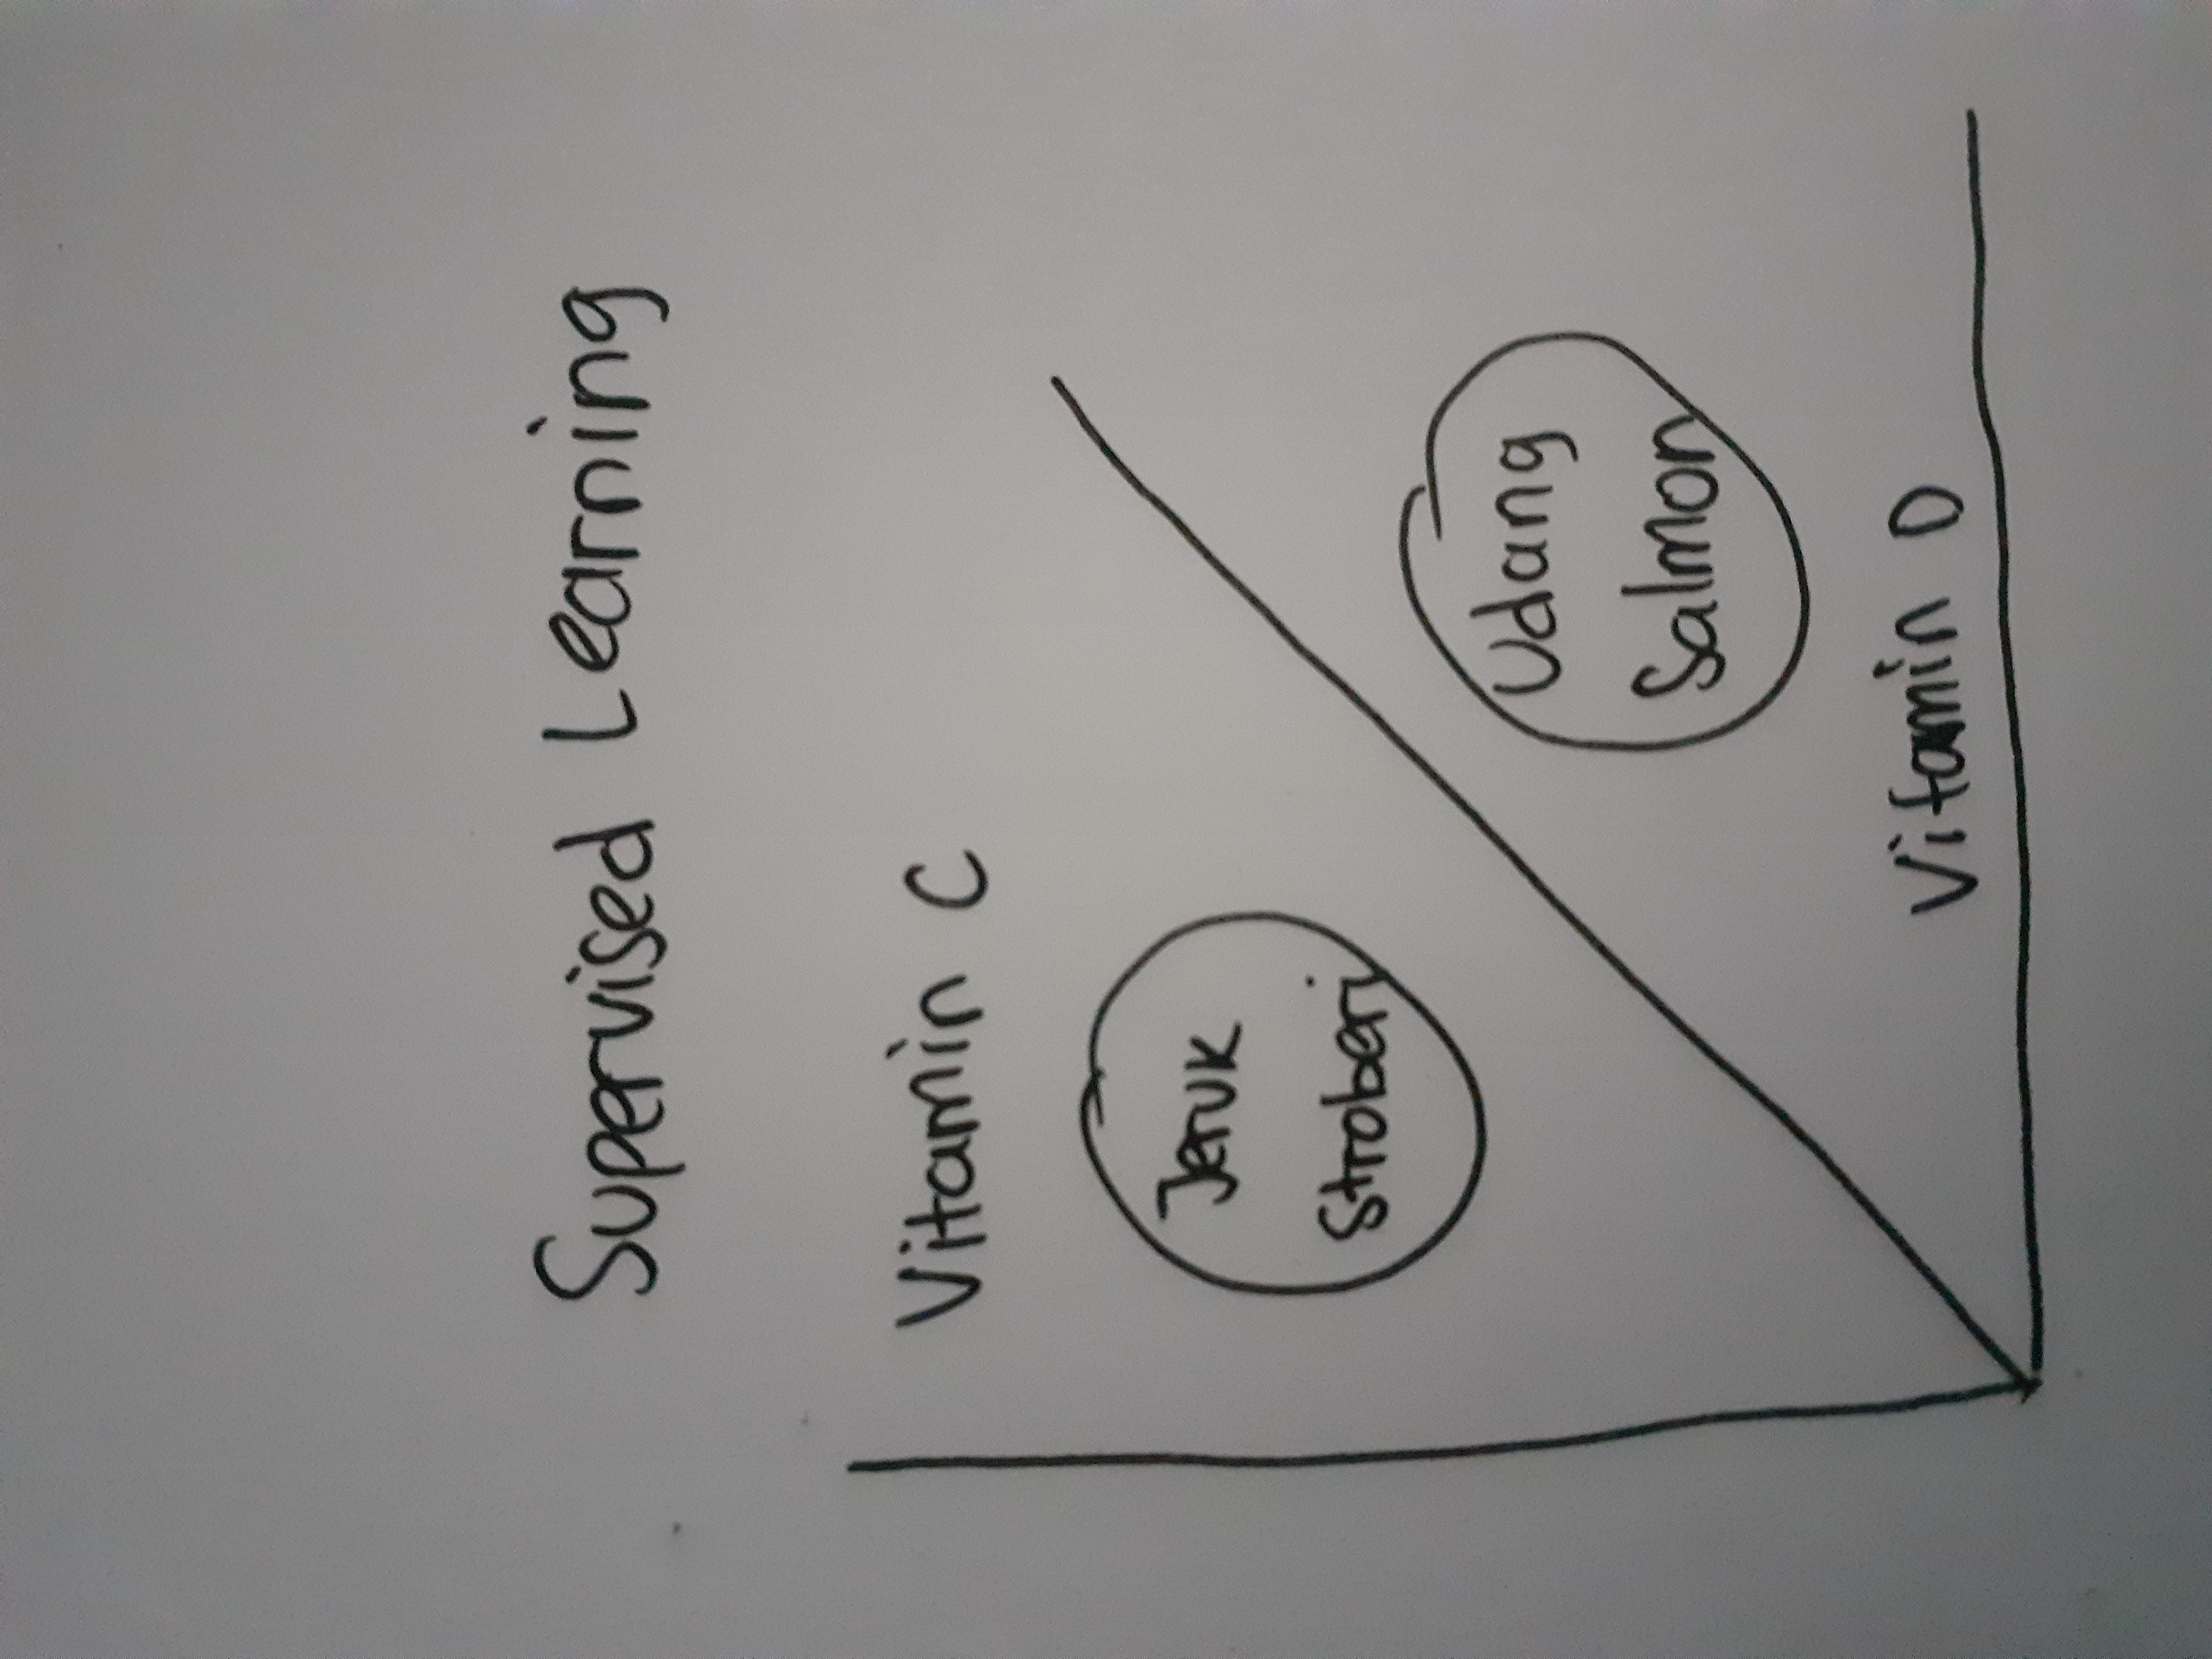
\includegraphics[scale=0.01]{figures/1174043/chapter2/2.jpg}
			\caption{contoh supervised learning}
			\label{contoh}
		\end{figure}
		
		Sedangkan unsupervised learning tidak memiliki data latih, sehinggga dari data yang ada, kita mengelompokan data tersebut menjadi dua bagian atau bahkan tiga bagian dan seterusnya. contoh Salmon di kategorikan ke dalam vitamin d untuk lebih jelasnya dapat dilihat pada gambar.\par
		\begin{figure}[ht]
			\centering
			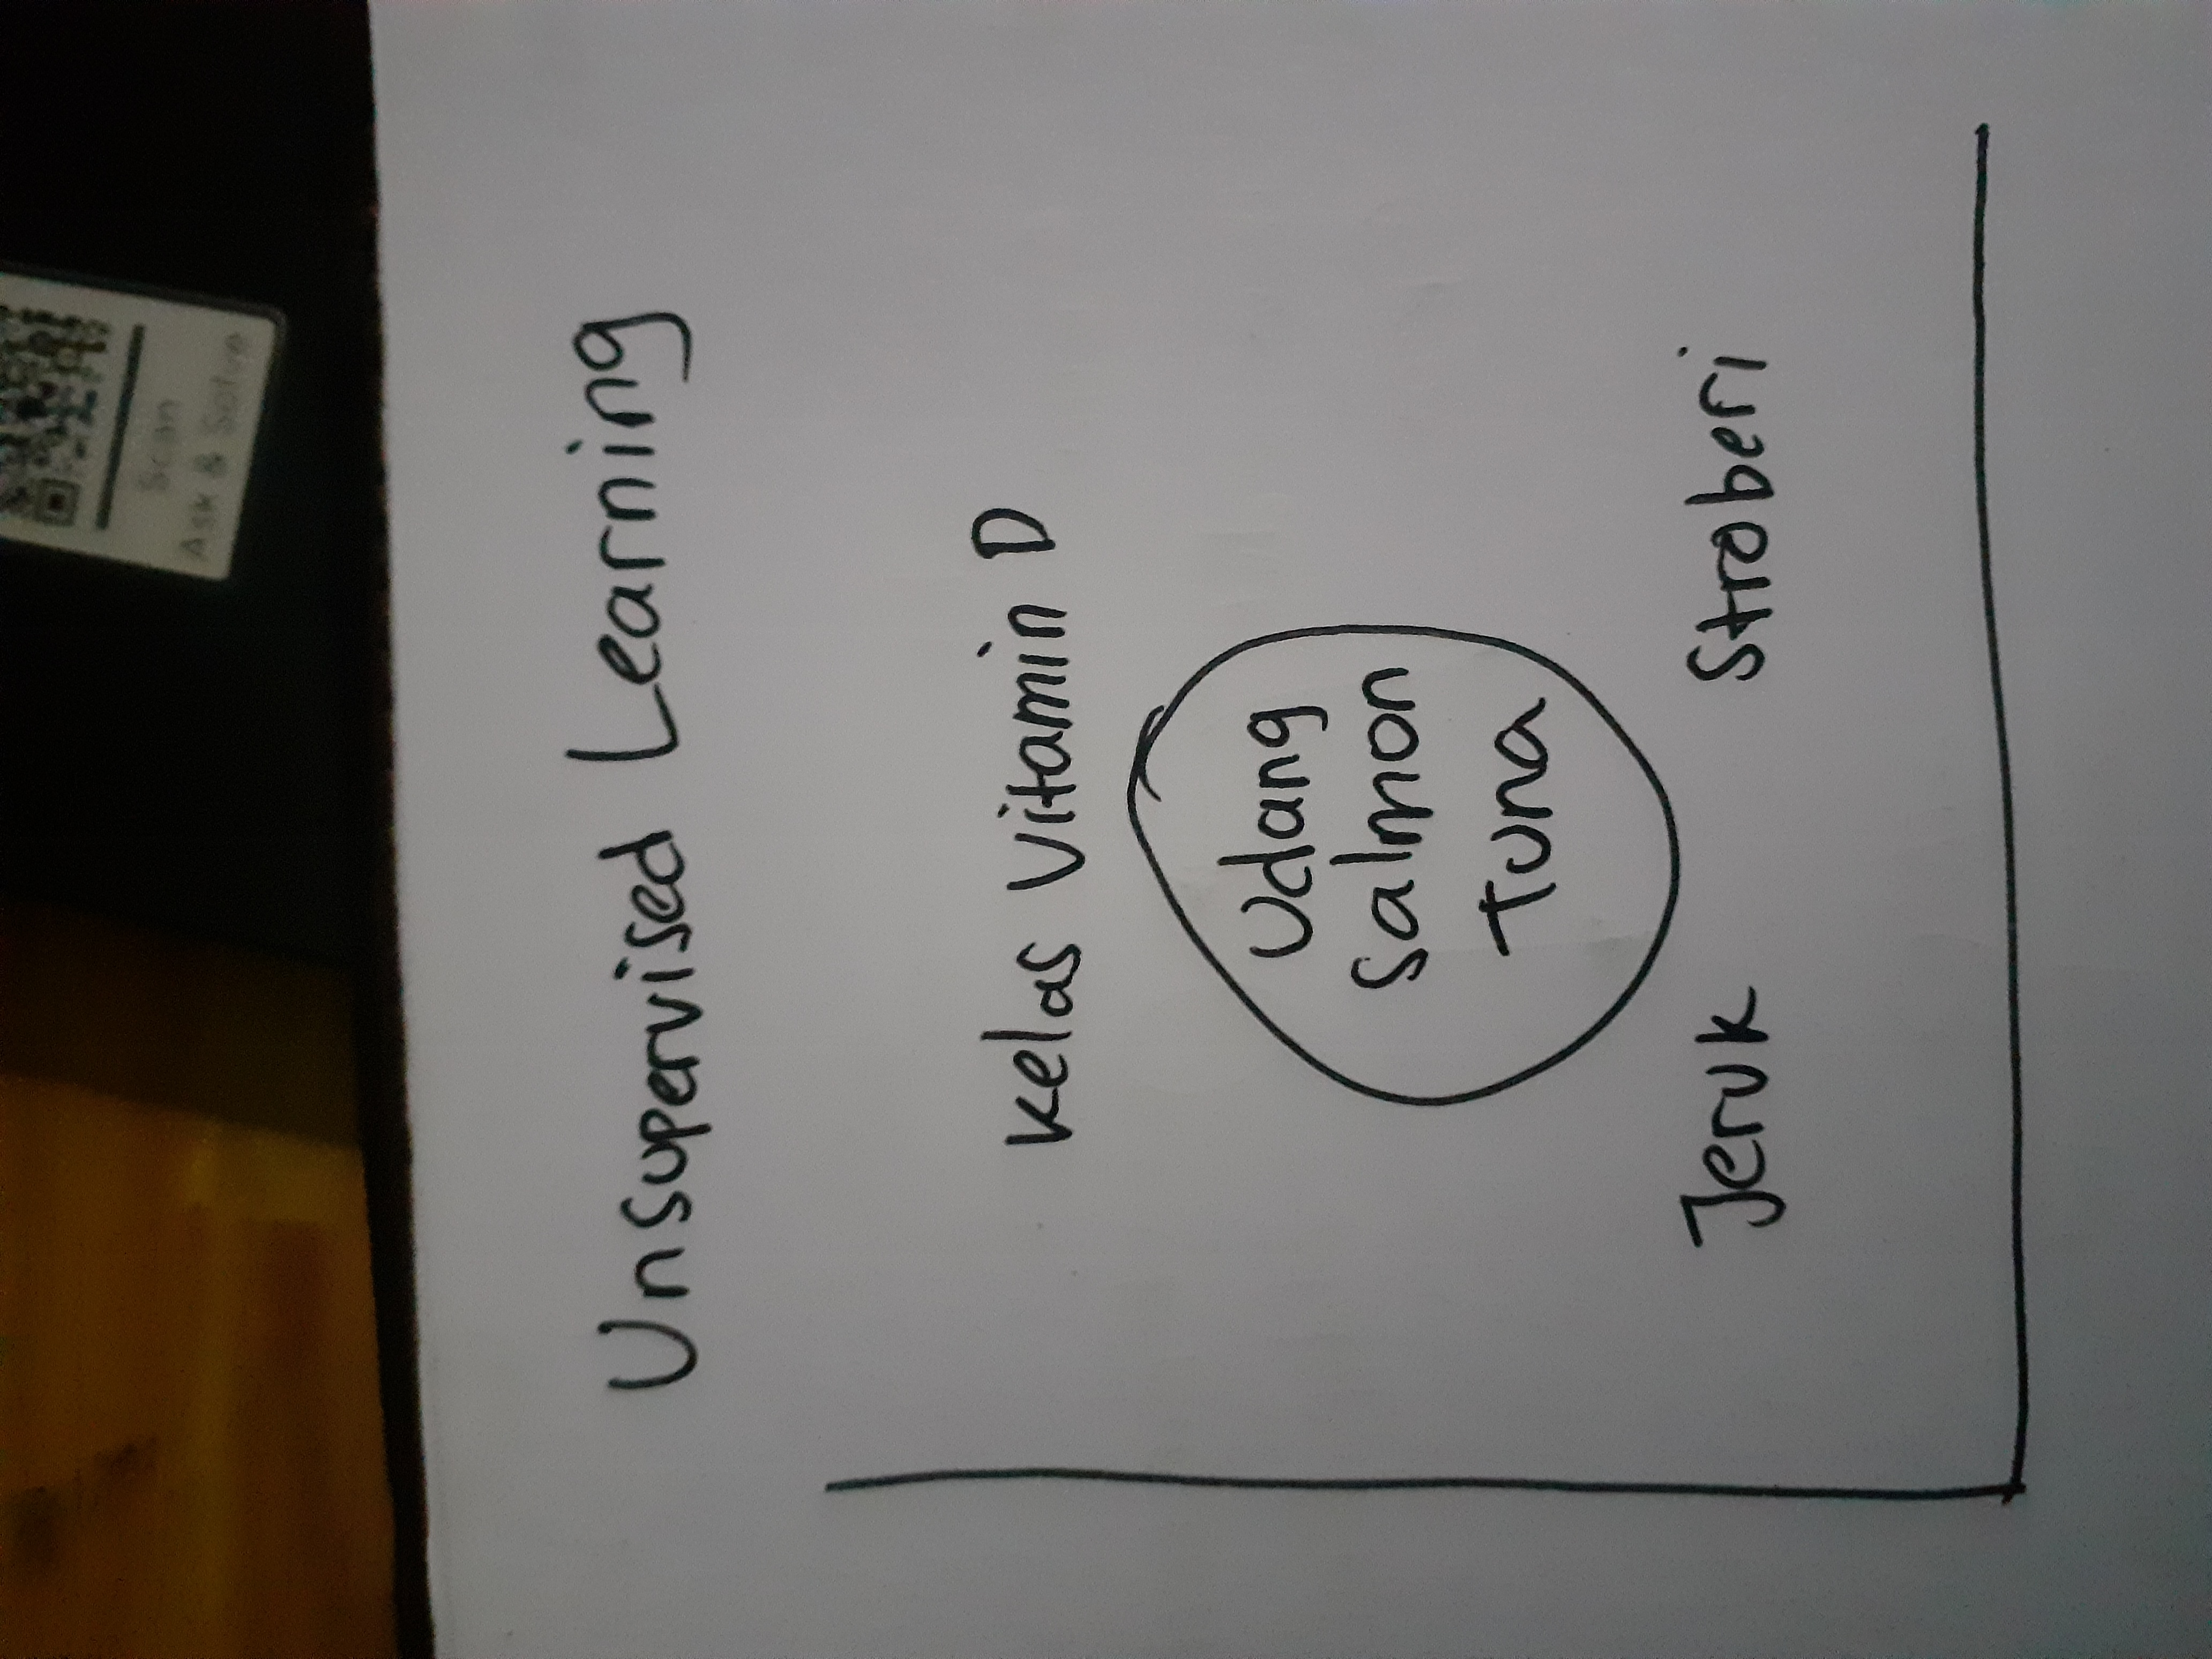
\includegraphics[scale=0.01]{figures/1174043/chapter2/3.jpg}
			\caption{contoh unsupervised learning}
			\label{contoh}
		\end{figure}
		
		clustering merupakan peroses mengklasifikasikan yang berdasarkan suatu parameter dalam penentuannya contoh pada berat vitamin c memiliki berat 500 gr dan vitamin d memiliki berat 1000 gr yang berarti berat dibagi dua parameter yaitu lebih kecil samadengan 500 gram dan lebih besar dari 500 gram contoh pada gambar.\par
		\begin{figure}[ht]
			\centering
			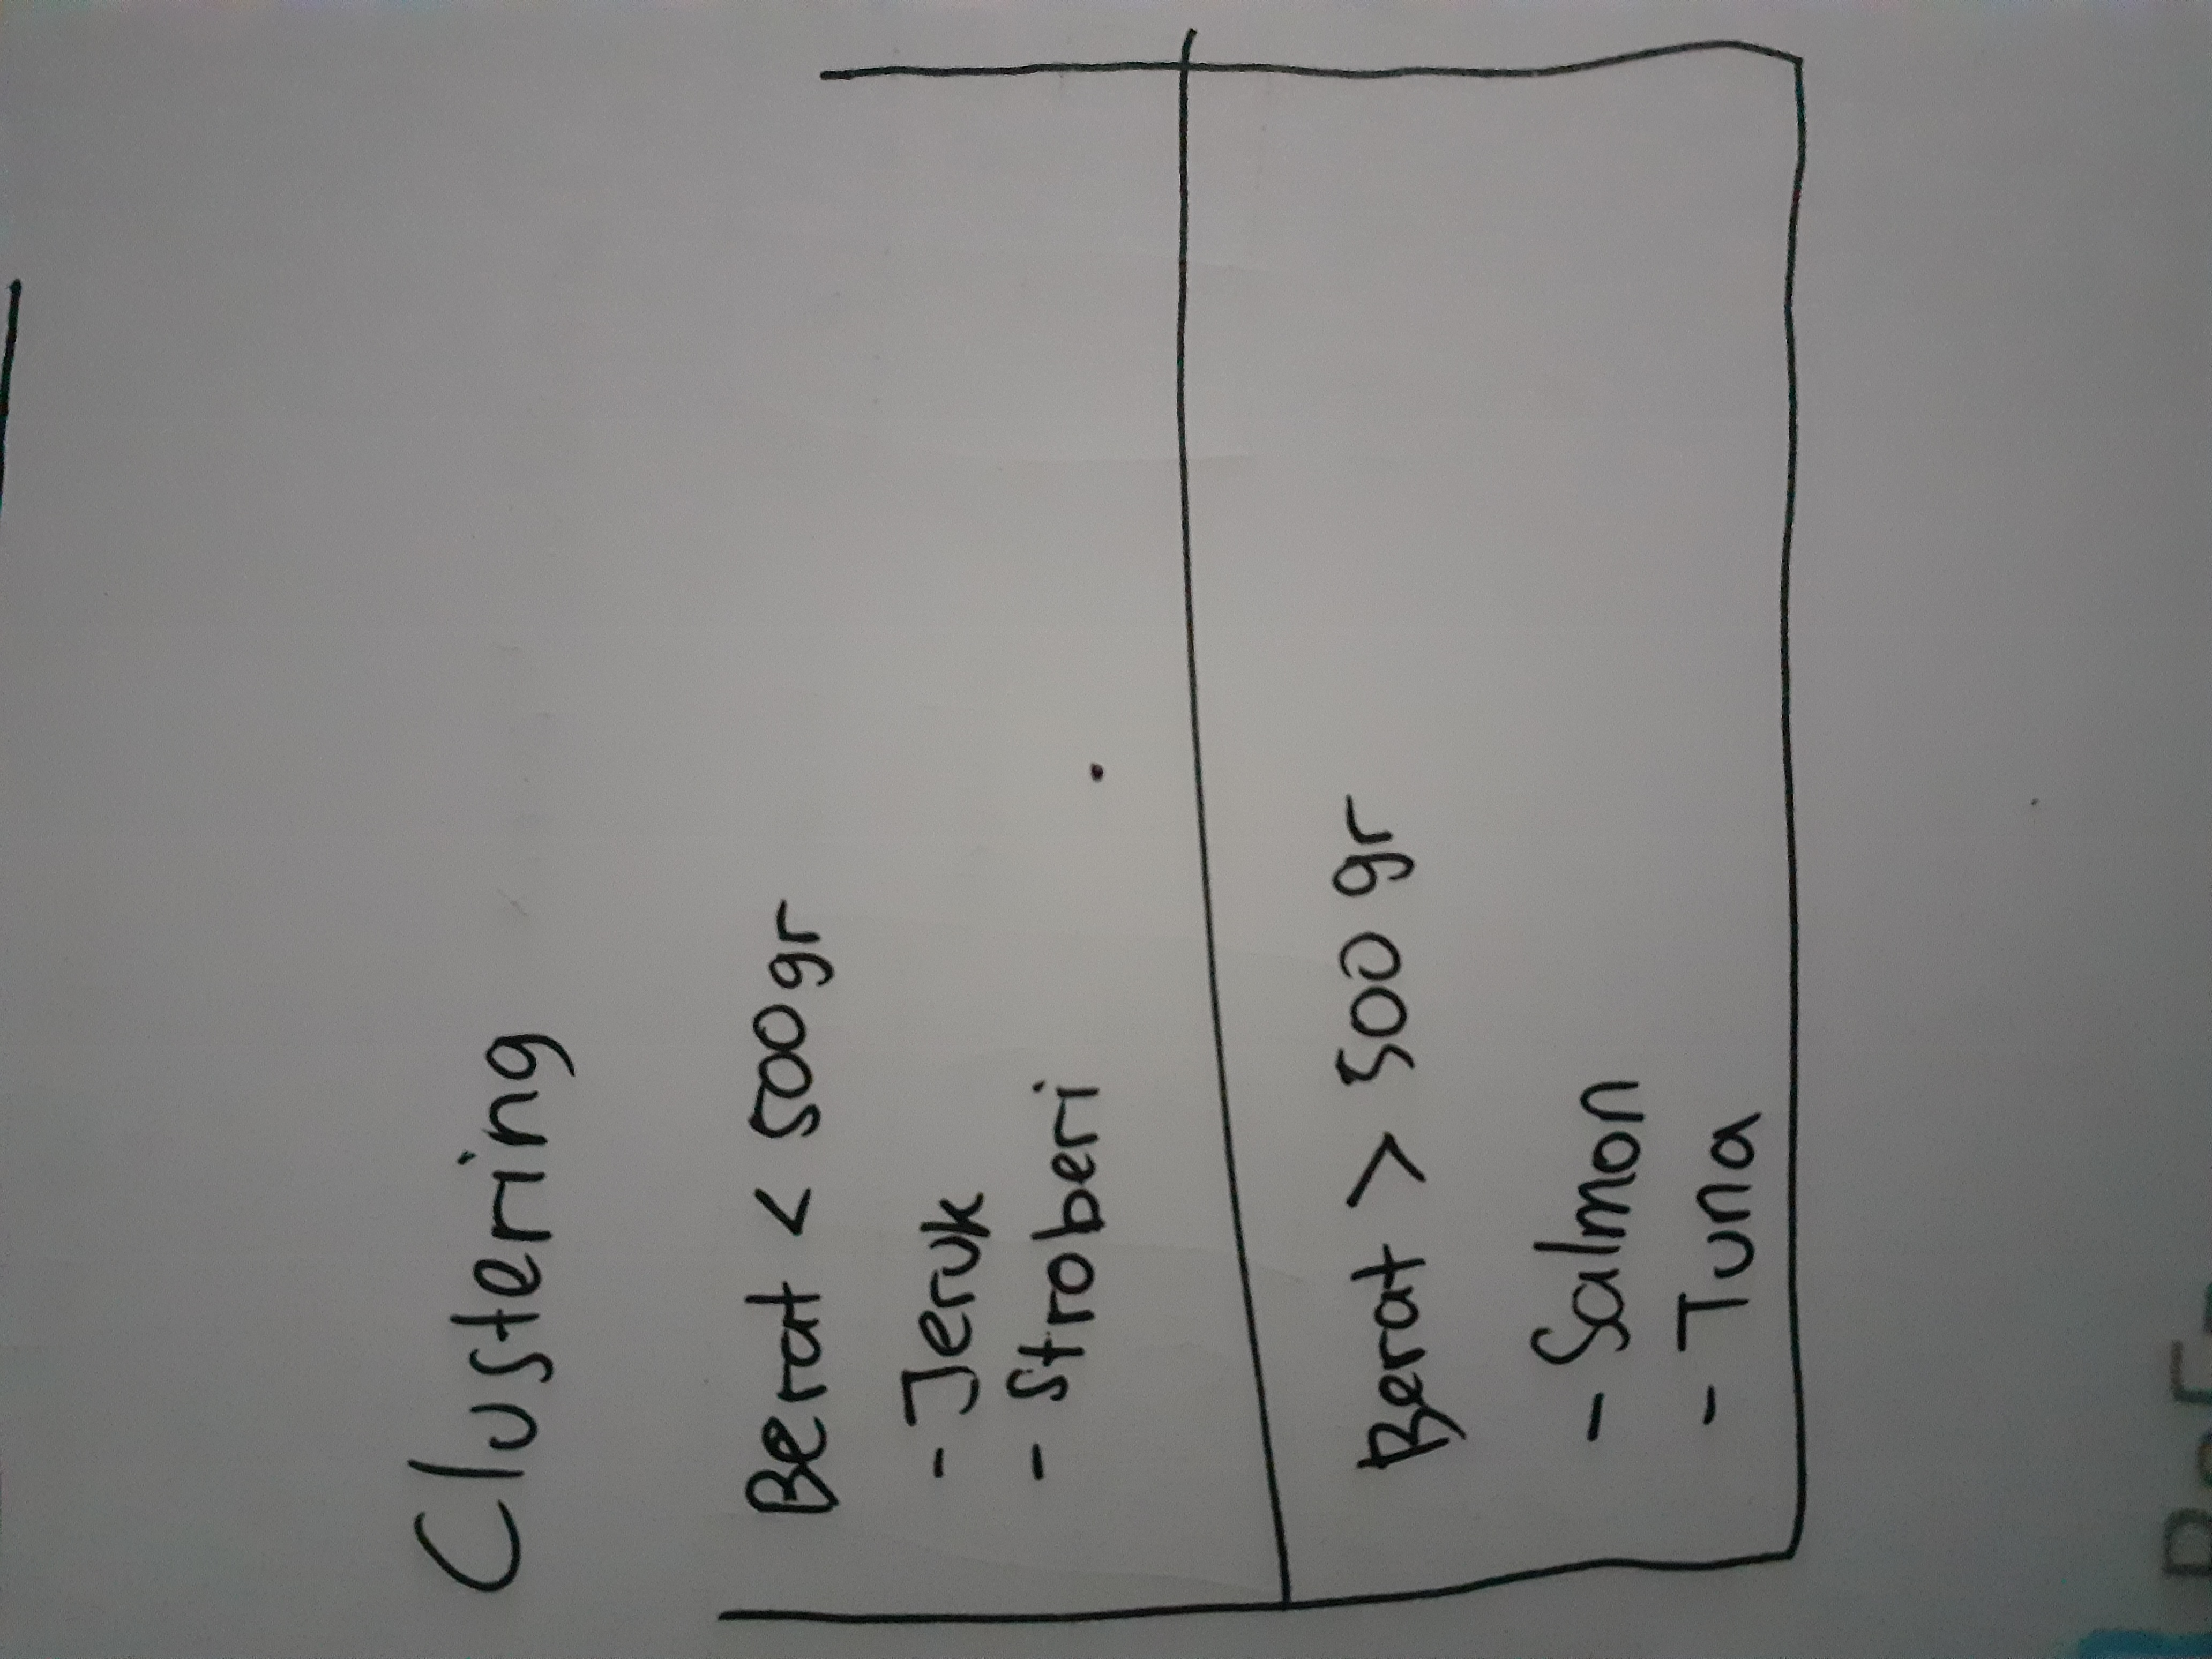
\includegraphics[scale=0.01]{figures/1174043/chapter2/4.jpg}
			\caption{contoh clustering}
			\label{contoh}
		\end{figure}
		
		\item Jelaskan apa itu evaluasi dan akurasi dan disertai ilustrasi contoh dengan gambar sendiri.\par
		evaluasi adalah pengumpulan pengumpulan dan pengamatan dari berbagai macam bukti untuk mengukur dampak efektifitas dari suatu objek, program, atau proses berkaitan  dengan spesifikasi atau persyaratan yang telah di tetapkan sebelumnya. sedangkan akurasi itu sndiri merupakan bagian dari evaluasi yang merupakan ketepatan data terhadap suatu objek berdasarkan keriteria tertentu. kita dappat mengevalluasi seberappa baik modell bekerja denggan menggukur akurasiinya. ketepatan akan di definisikan sebagai presentase kasus yang di klasifikasikan dengan benar. hal ini berkaitan dengan confusion matrix pada materi selanjutnya.lebih jelasnya pada gambar berikut:
		\begin{figure}[ht]
			\centering
			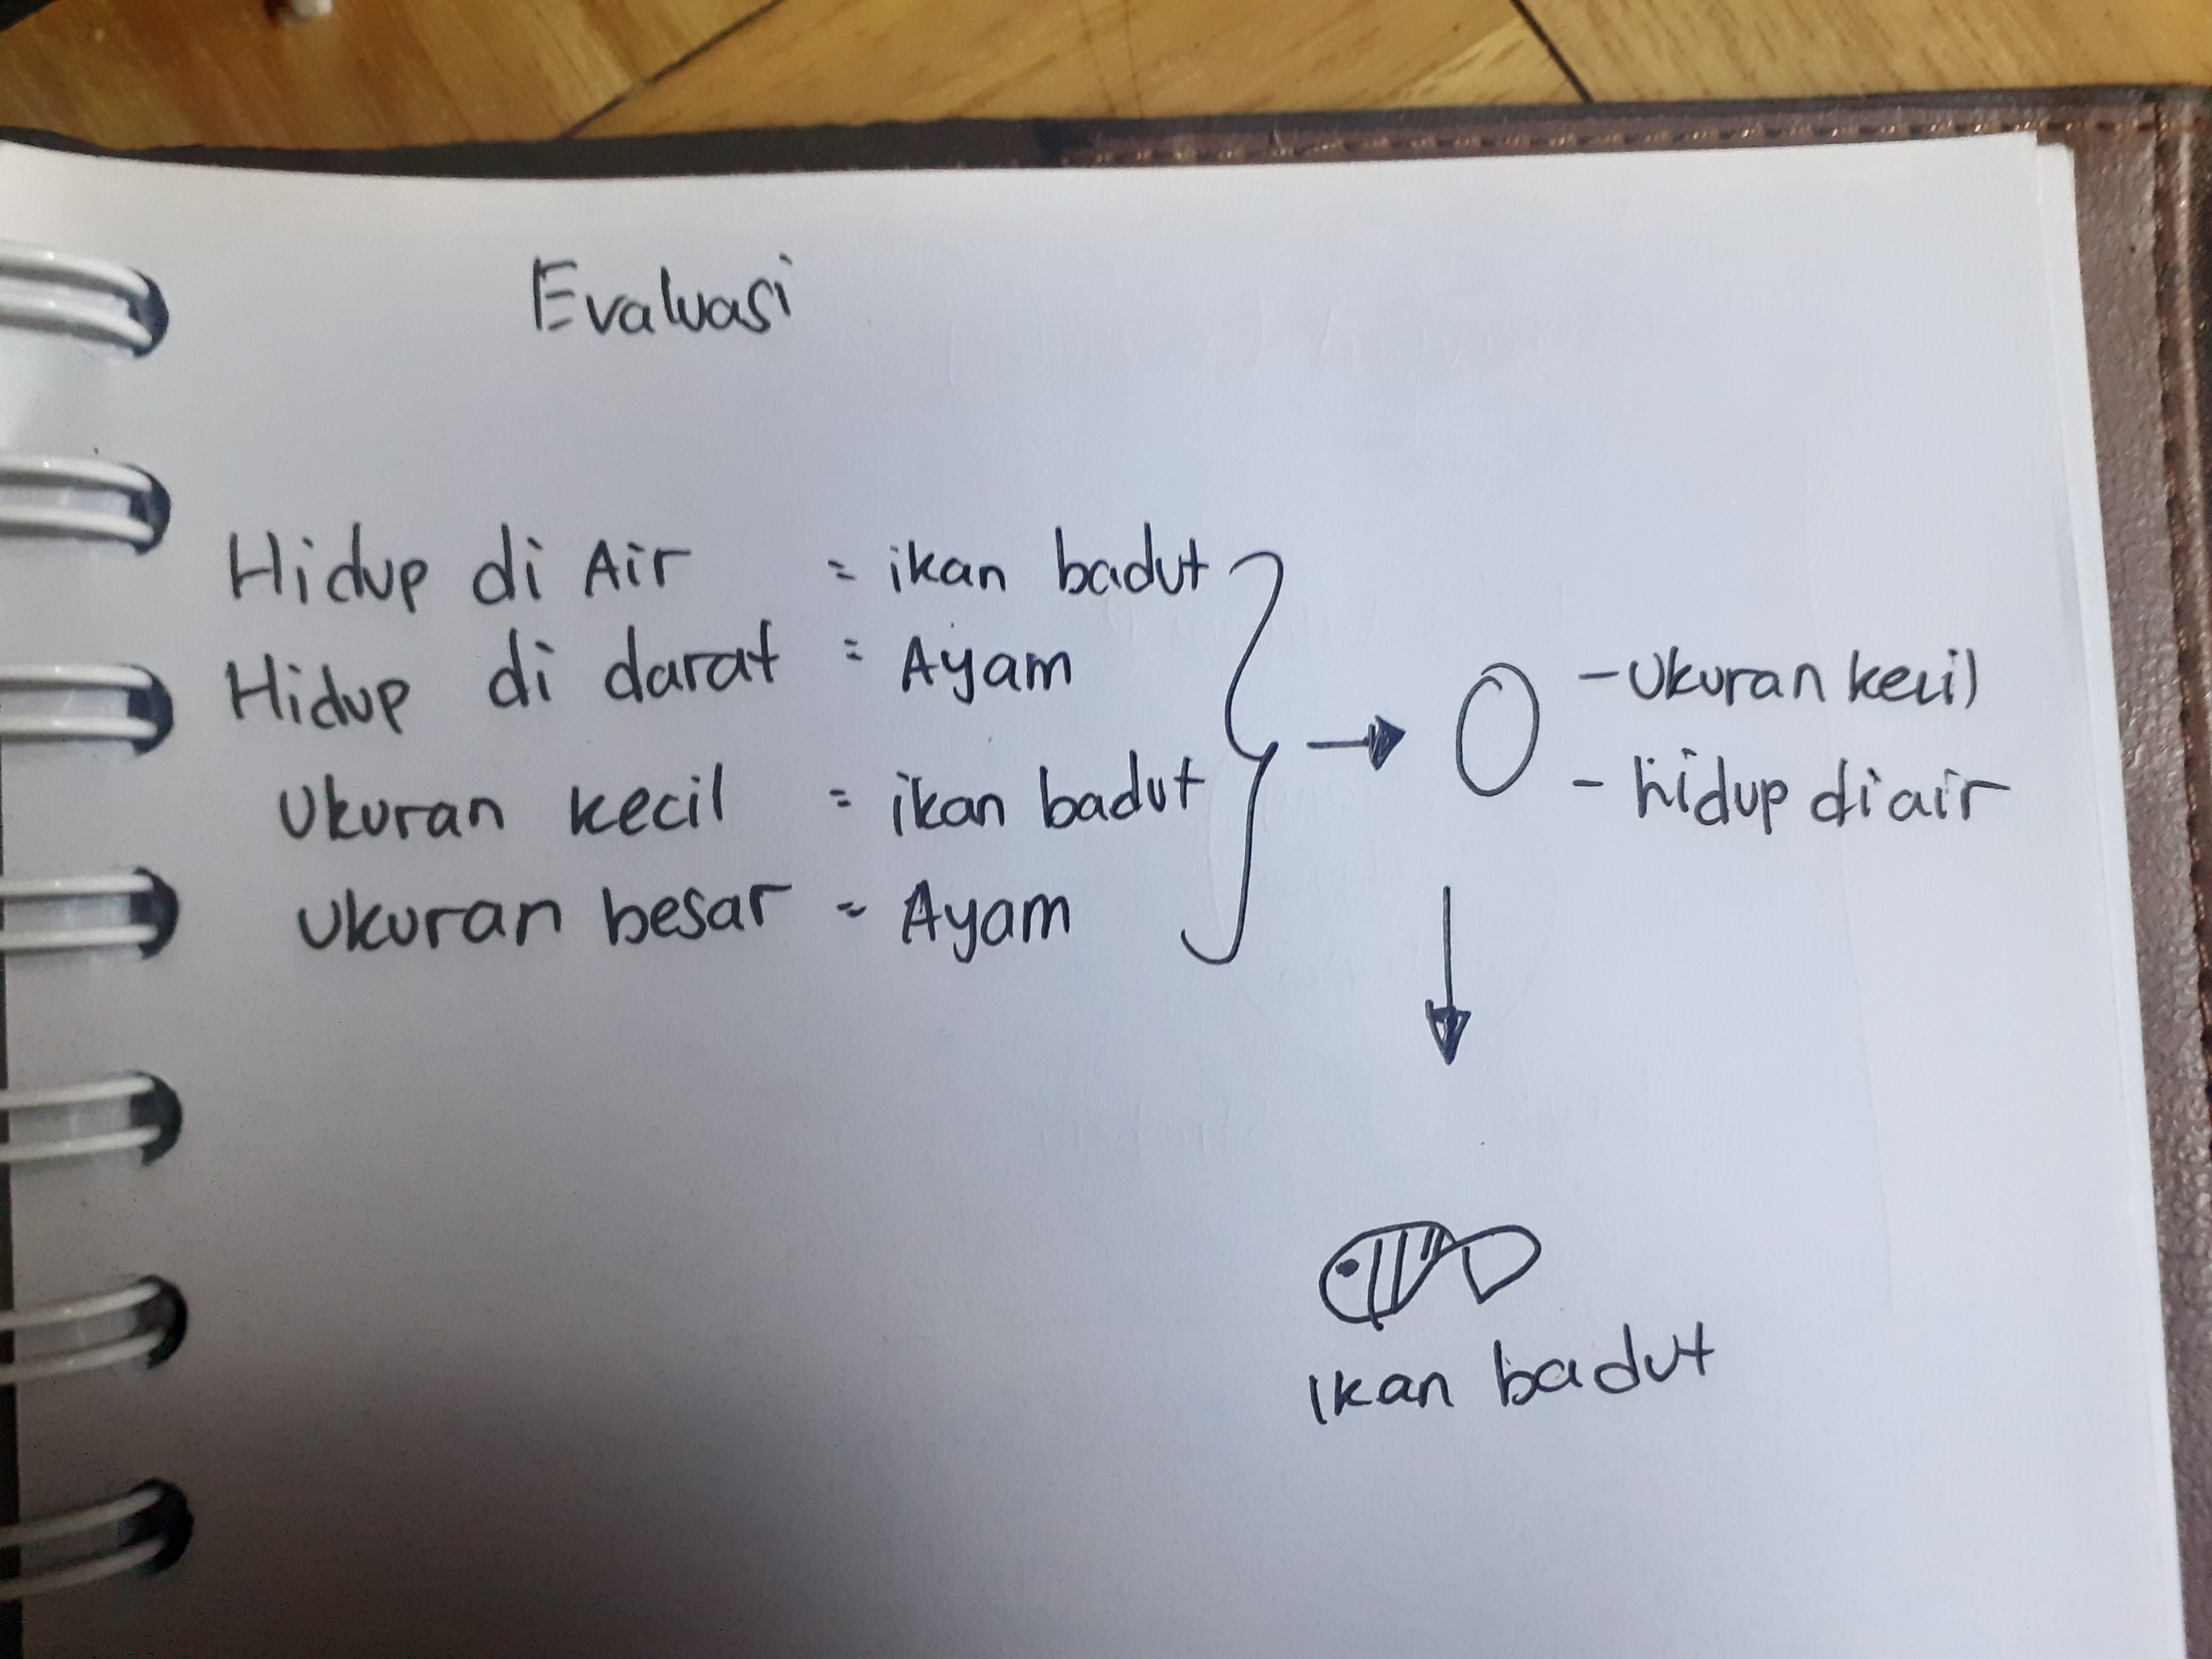
\includegraphics[scale=0.01]{figures/1174043/chapter2/5.jpg}
			\caption{contoh Evaluasi}
			\label{contoh}
		\end{figure}
		
		\item Jelaskan bagaimana cara membuat Confusion Matrix, Buat confusion matrix sendiri.\par
		Dalam pembuatan confusion matrix tentukan parameter atau objek yang akan di evaluasi contoh udang, salmon, tuna buat tabel dengan baris dan kolom berjumlah tiga kemudian tentukan nilai miring pada setiap kolom tersebut disini saya memberi nilai 20 dengan ketentuan setiap baris harus berisi nilai 20 nilai tersebut jika terbagi ke kolom lain maka jumlahnya harus bernilai 20 jika tidak berarti data tersebut tidak akurat. untuk lebih jelanya dapat dilihat pada gambar berikut :
		\begin{figure}[ht]
			\centering
			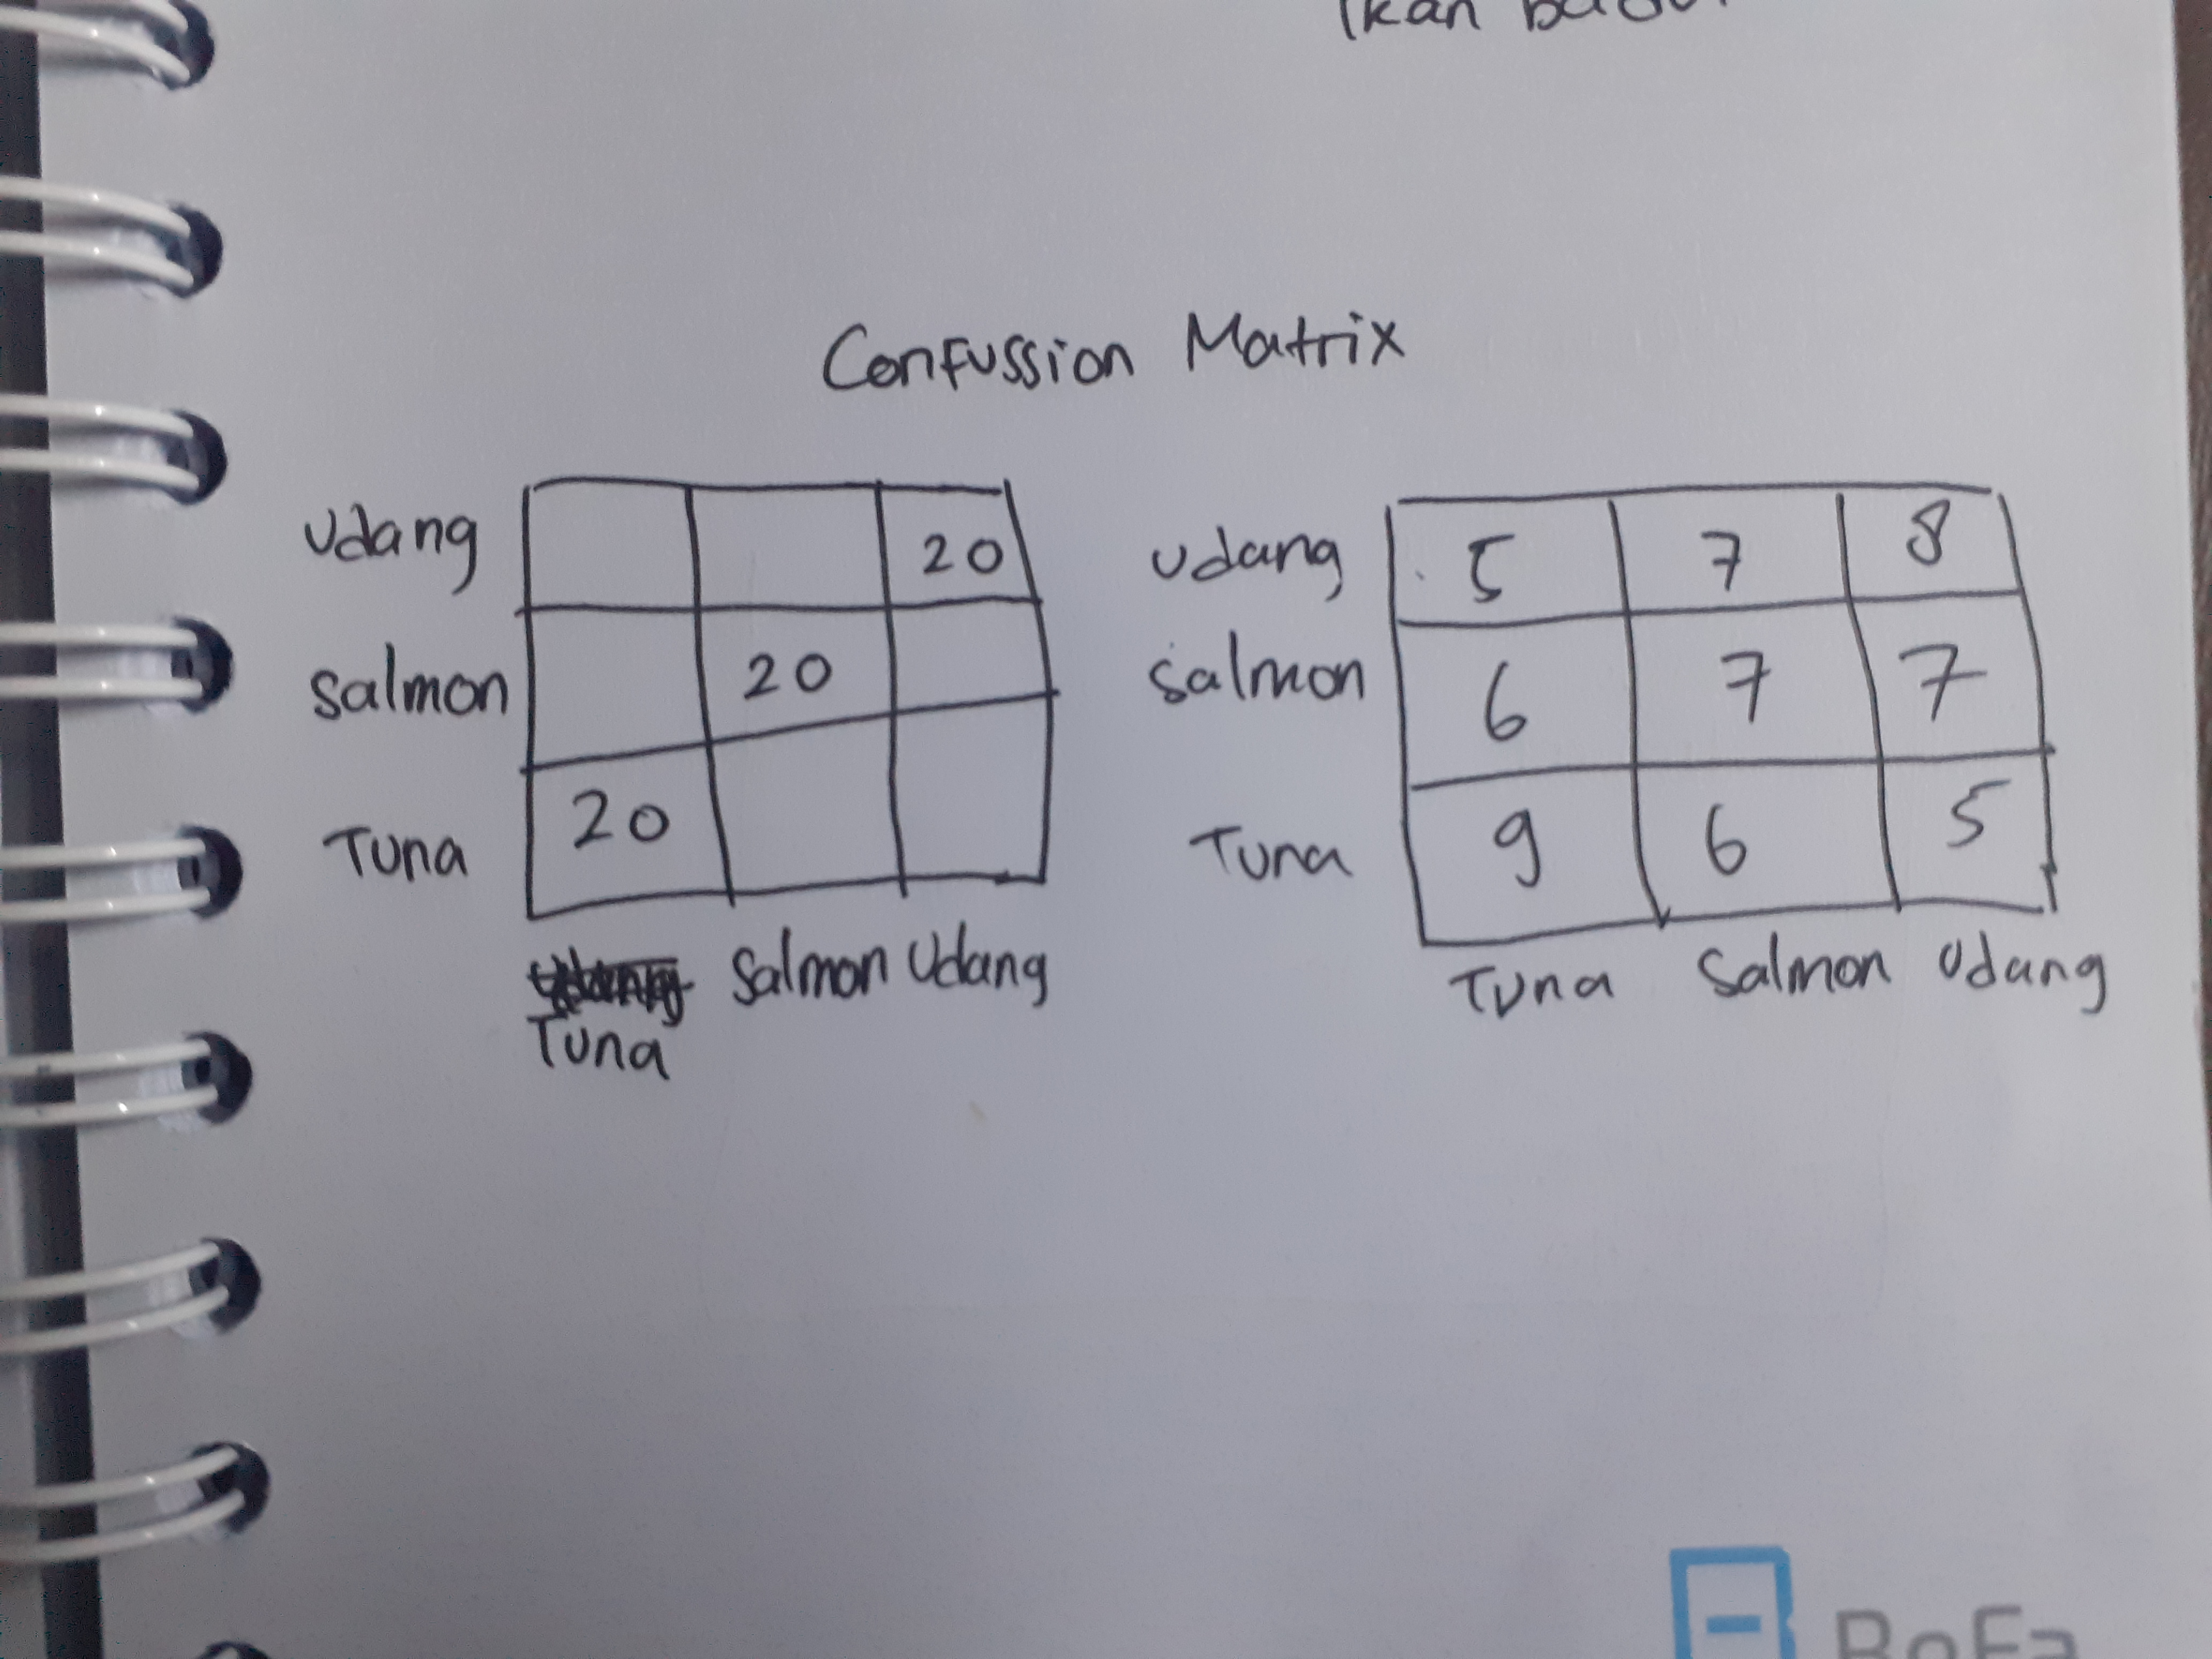
\includegraphics[scale=0.01]{figures/1174043/chapter2/6.jpg}
			\caption{contoh Confusion Matrix}
			\label{contoh}
		\end{figure}
		
		\item Jelaskan bagaimana K-fold cross validation bekerja dengan gambar ilustrasi contoh buatan sendiri. \par
		K-fold Cross Validation merupakan cara untuk melatih suatu mesin dimana di dalammya terdapat data set yang dibagi menjadi dua yaitu untuk data testing dan data training contoh 1000 data merupakan data set dan 400 data digunakan untuk data testing kemudian 600 datanya digunakan untuk data training dimana data training tersebut digunakan untuk menentukan nilai bobot yang dimasukan kedalam rumus regresi linier. sedangkan nilai testing akan dijadikan nili inputan untuk rumus regresi linier. contohnya dapat dilihat pada gambar berikut :
		\begin{figure}[ht]
			\centering
			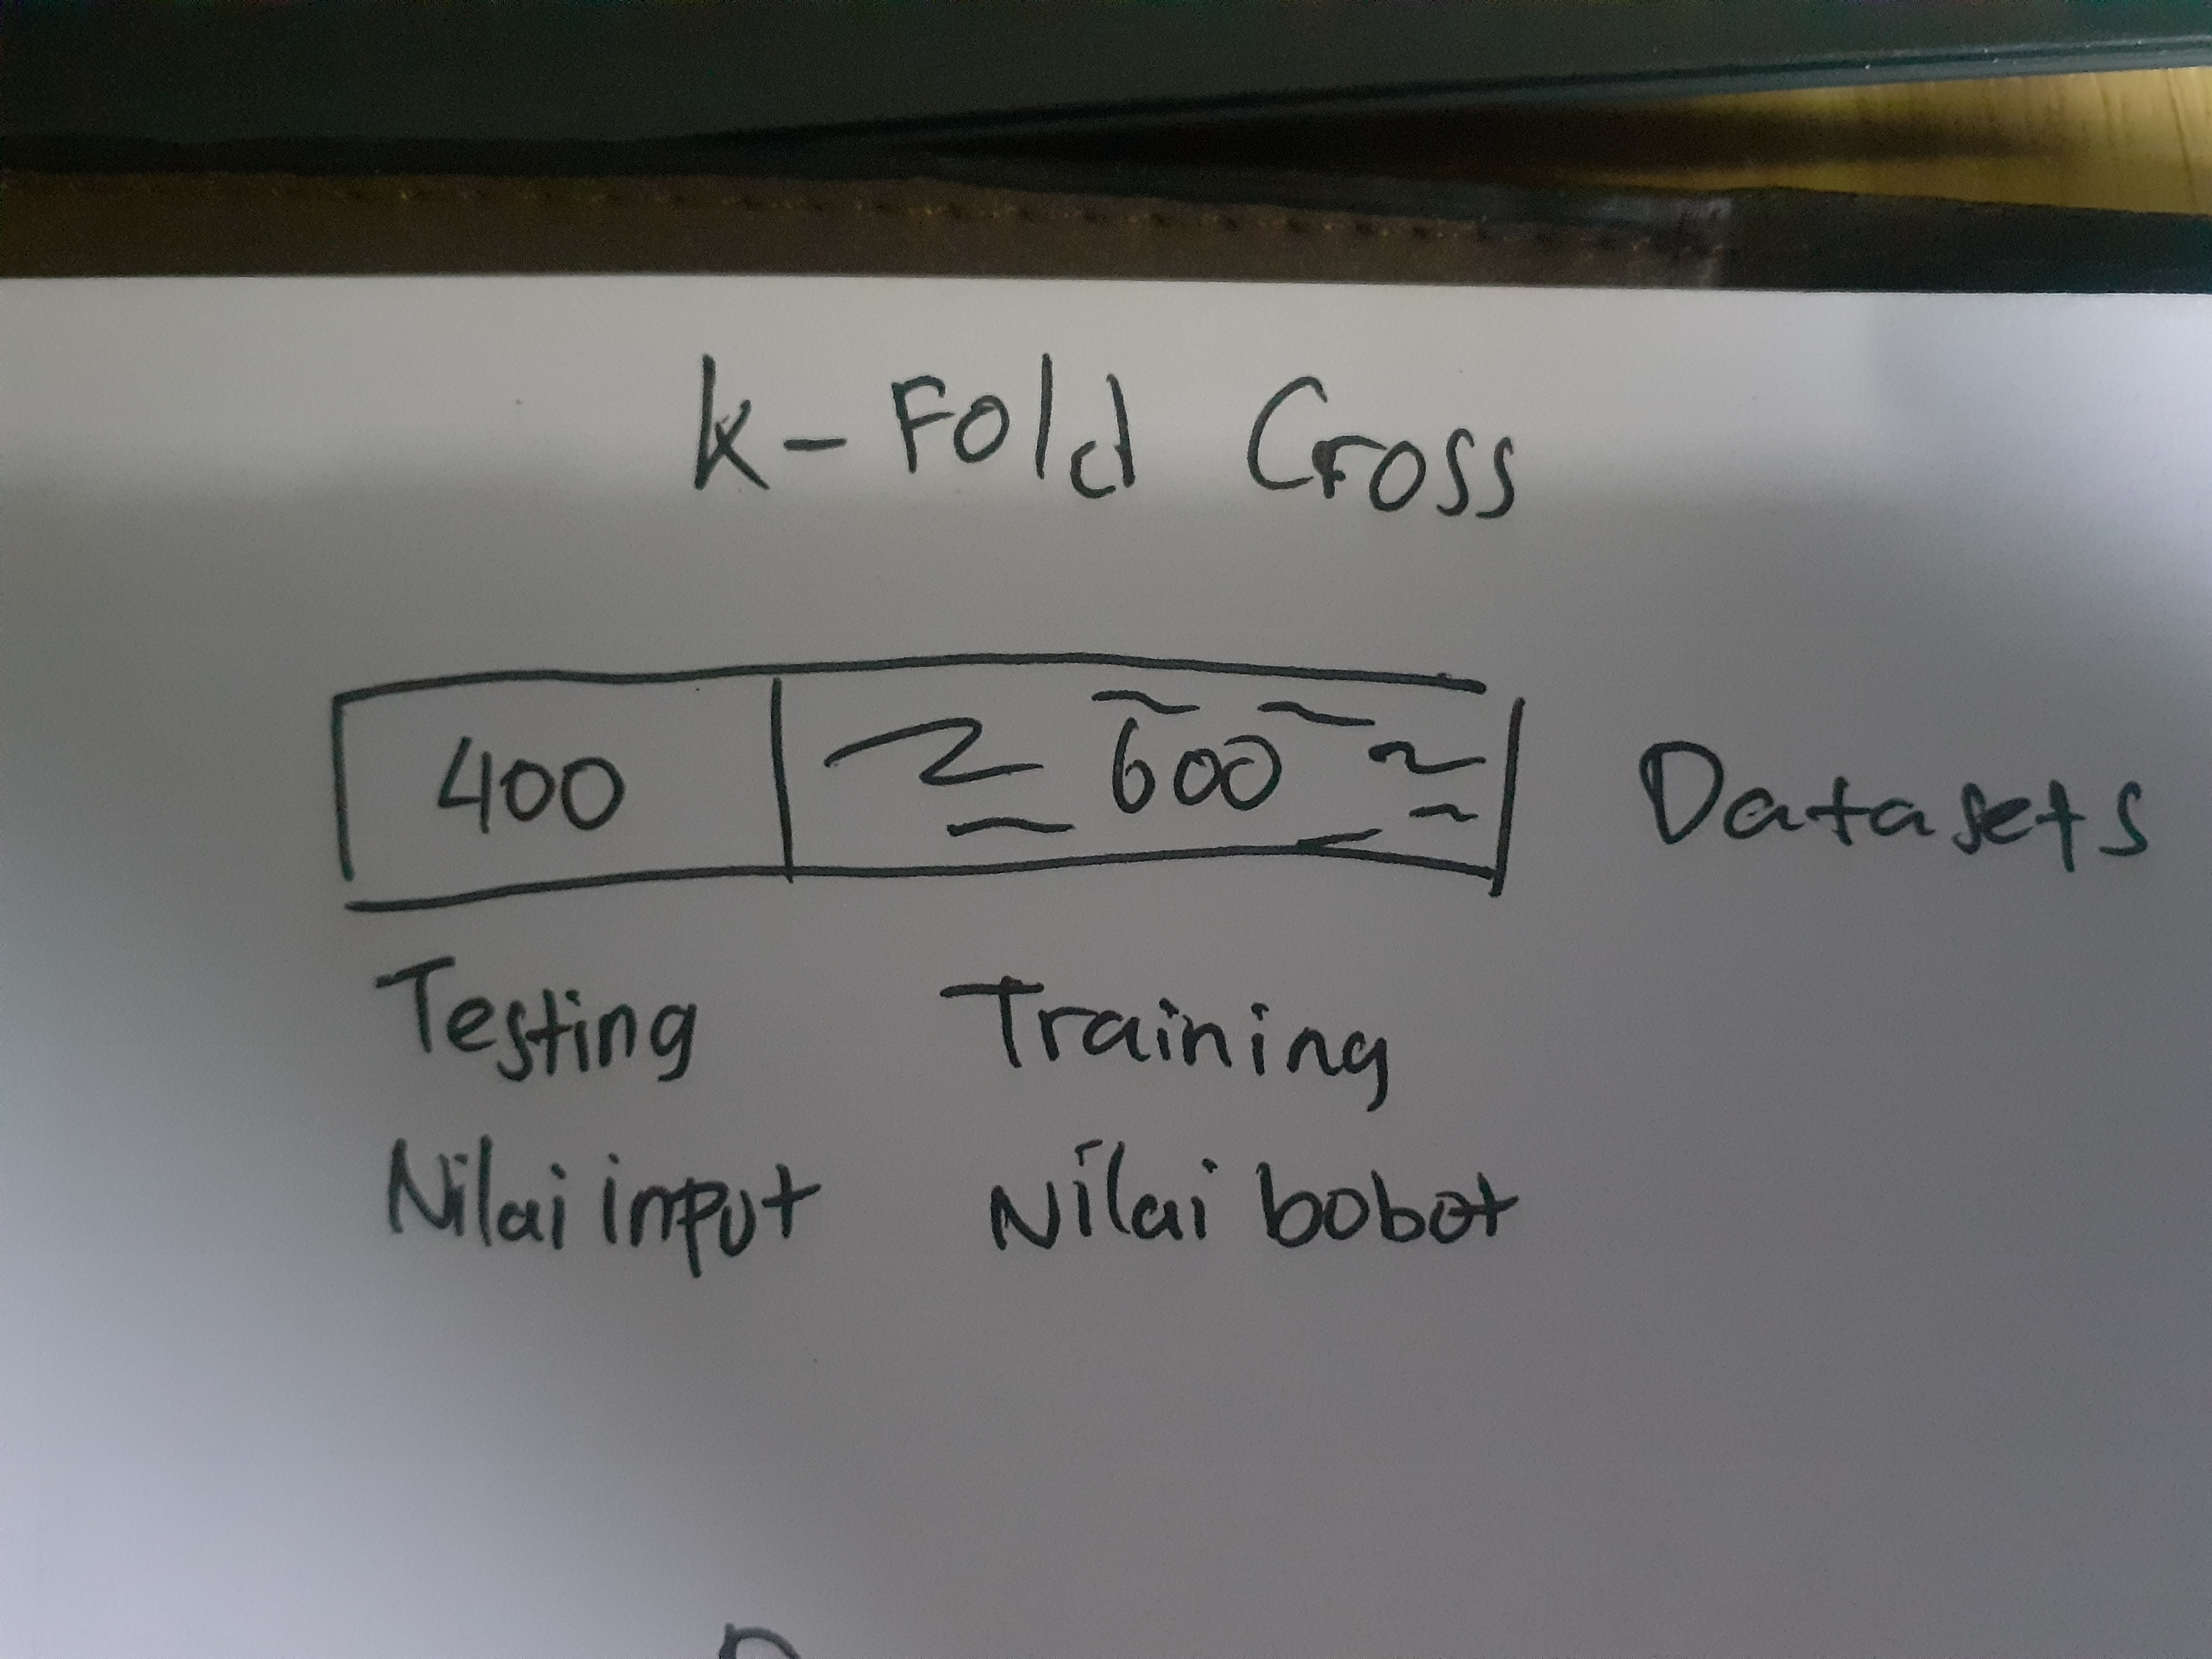
\includegraphics[scale=0.01]{figures/1174043/chapter2/7.jpg}
			\caption{contoh K-fold cross validation}
			\label{contoh}
		\end{figure}
		
		\item Jelaskan Apa itu decision tree dengan gambar ilustrasi contoh buatan sendiri.\par
		Decision tree merupakan implementasi dari binari clasification dimana pada pohon keputusan akan terdapat root atau akar dan cabang cabangnya yang nilainya seperti if contoh pada root berisi nilai hewan hidup di air, apakah ikan pada cabang satu bernilai iya dan pada cabang dua bernilai tidak jika nilainya iya berarti hidup di air dan jika tidak maka bukan hidup diair.
		\begin{figure}[ht]
			\centering
			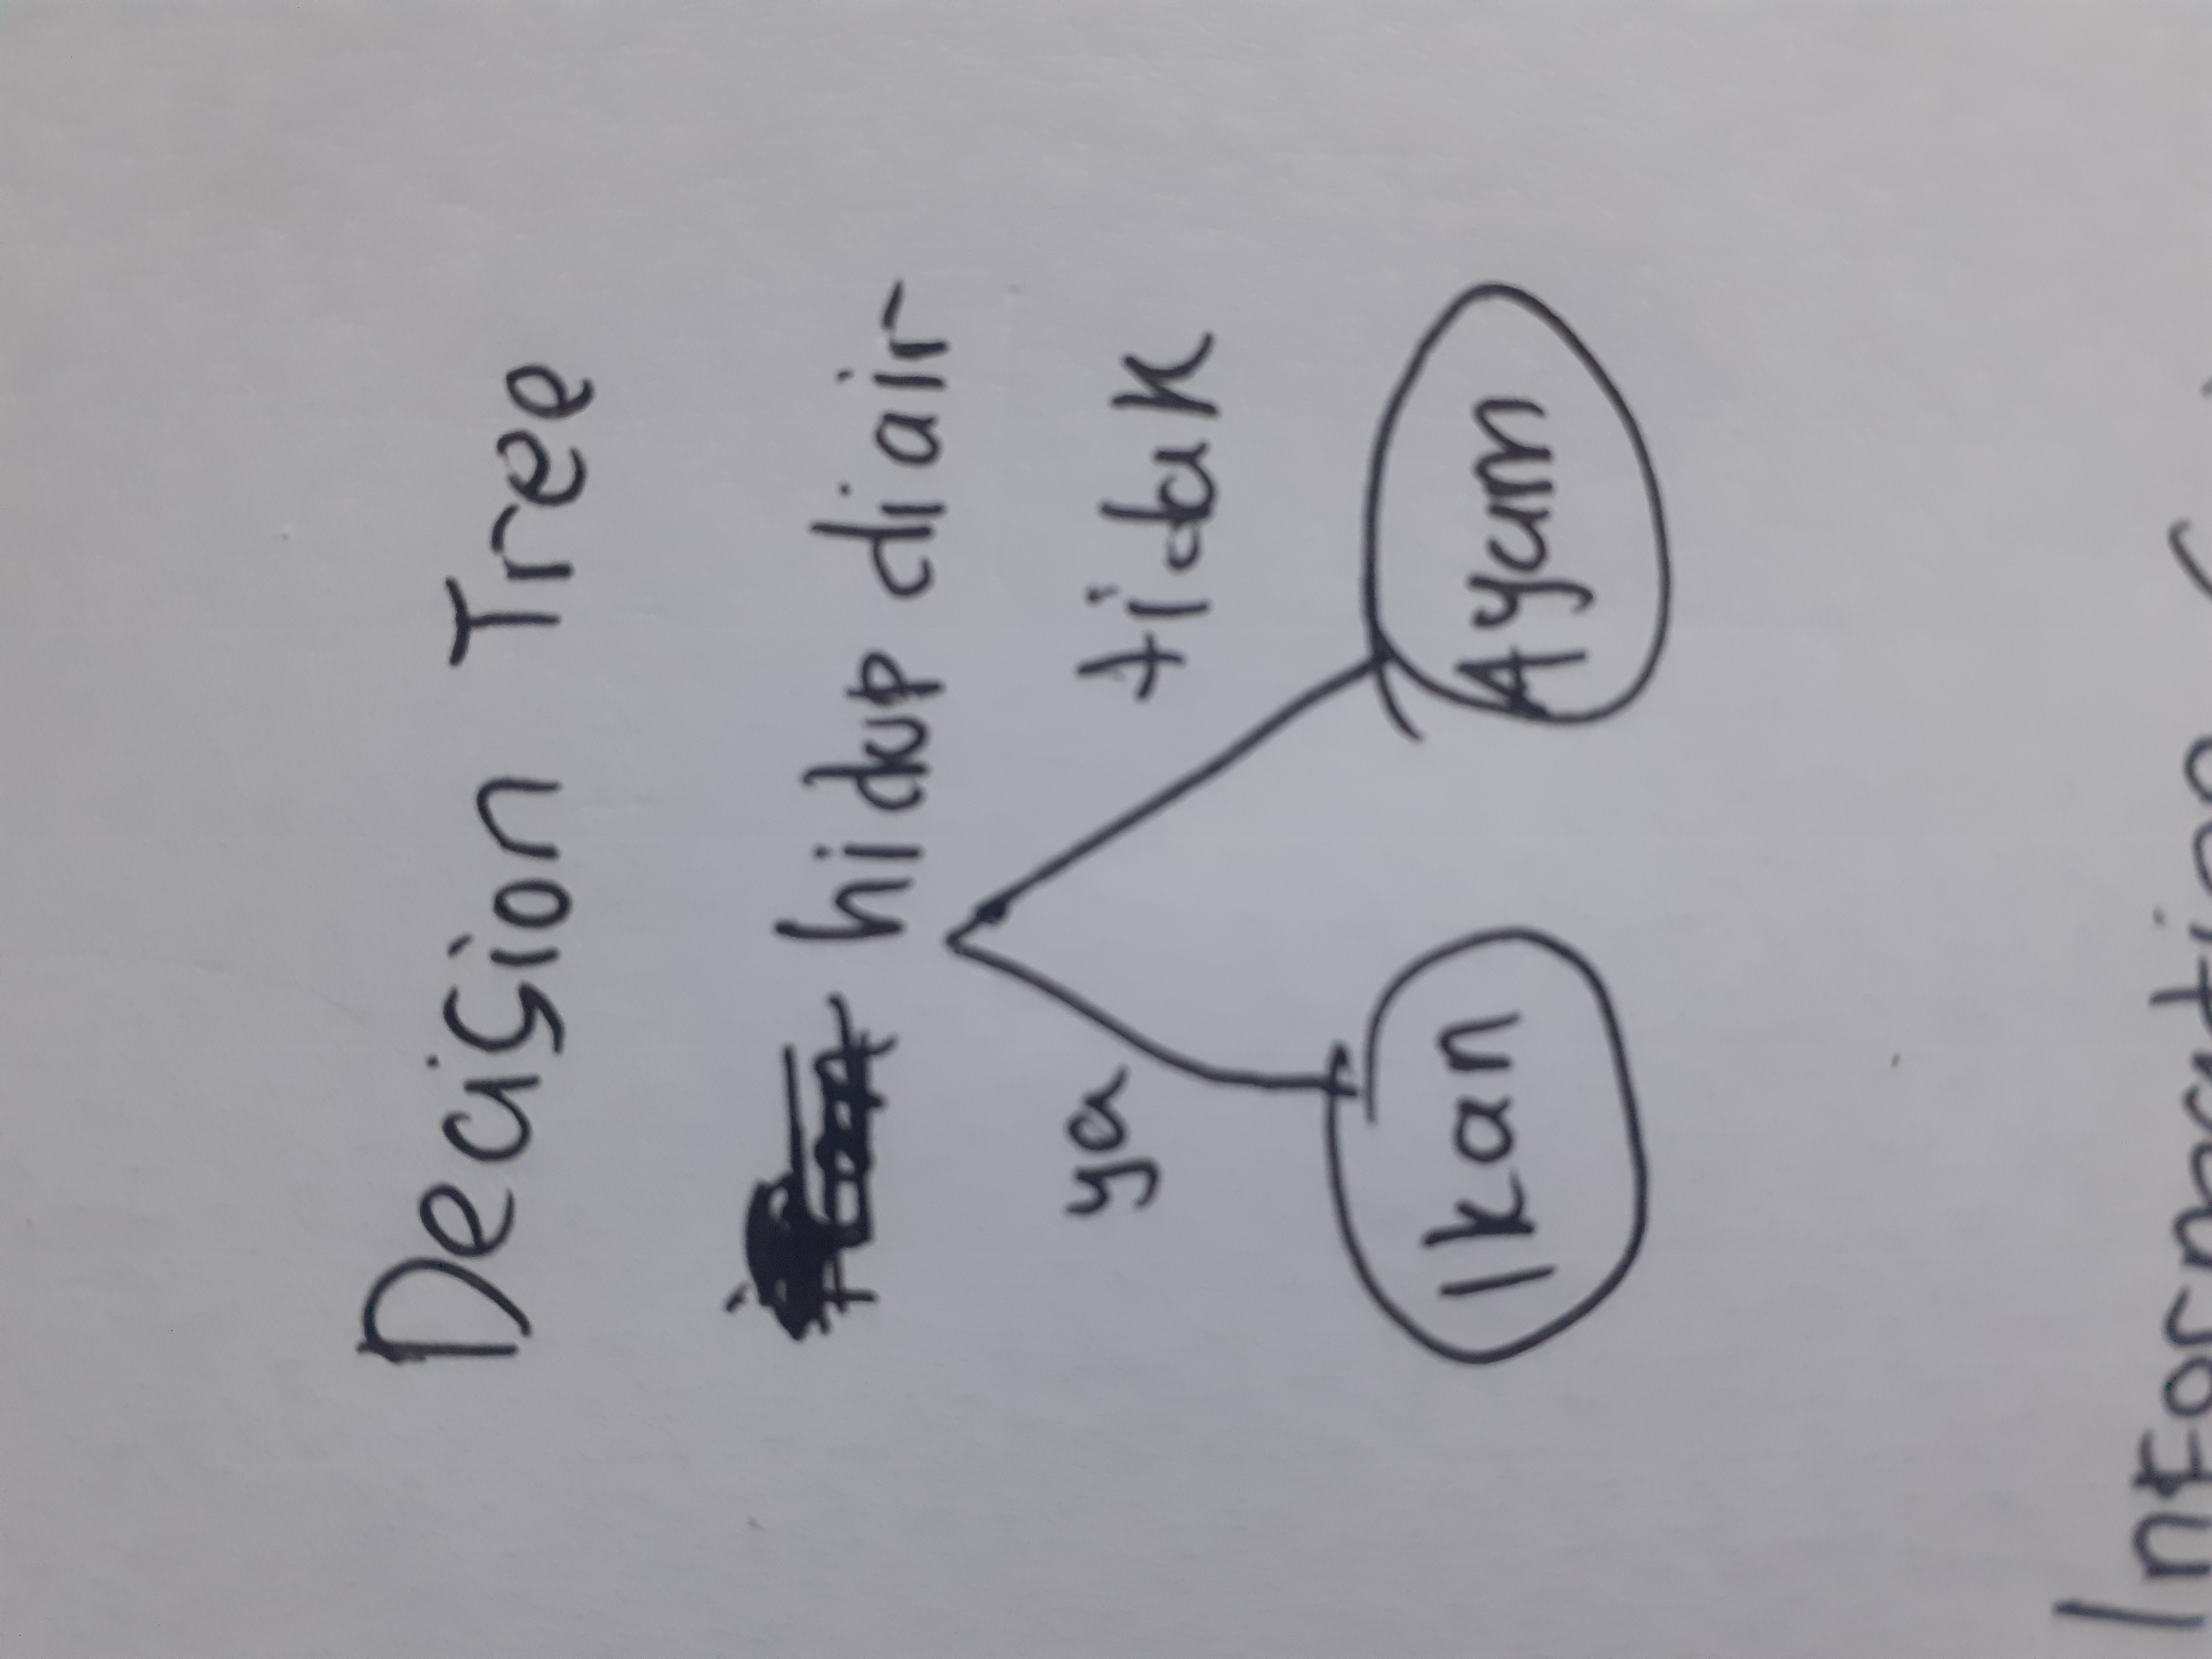
\includegraphics[scale=0.01]{figures/1174043/chapter2/8.jpg}
			\caption{contoh decision tree}
			\label{contoh}
		\end{figure}
		
		\item jelaskan apa itu information gain dan entropi dengan gambar ilustrasi buatan sendiri.\par
		informasion gain merupakan informasi atau keriteria dalam pembagian sebuah objek contoh information gain pada ikan yaitu hidup di air, berkoloni, berinsang. untuk lebih jelasnya dapat dilihat pada gambar berikut :\par
		\begin{figure}[ht]
			\centering
			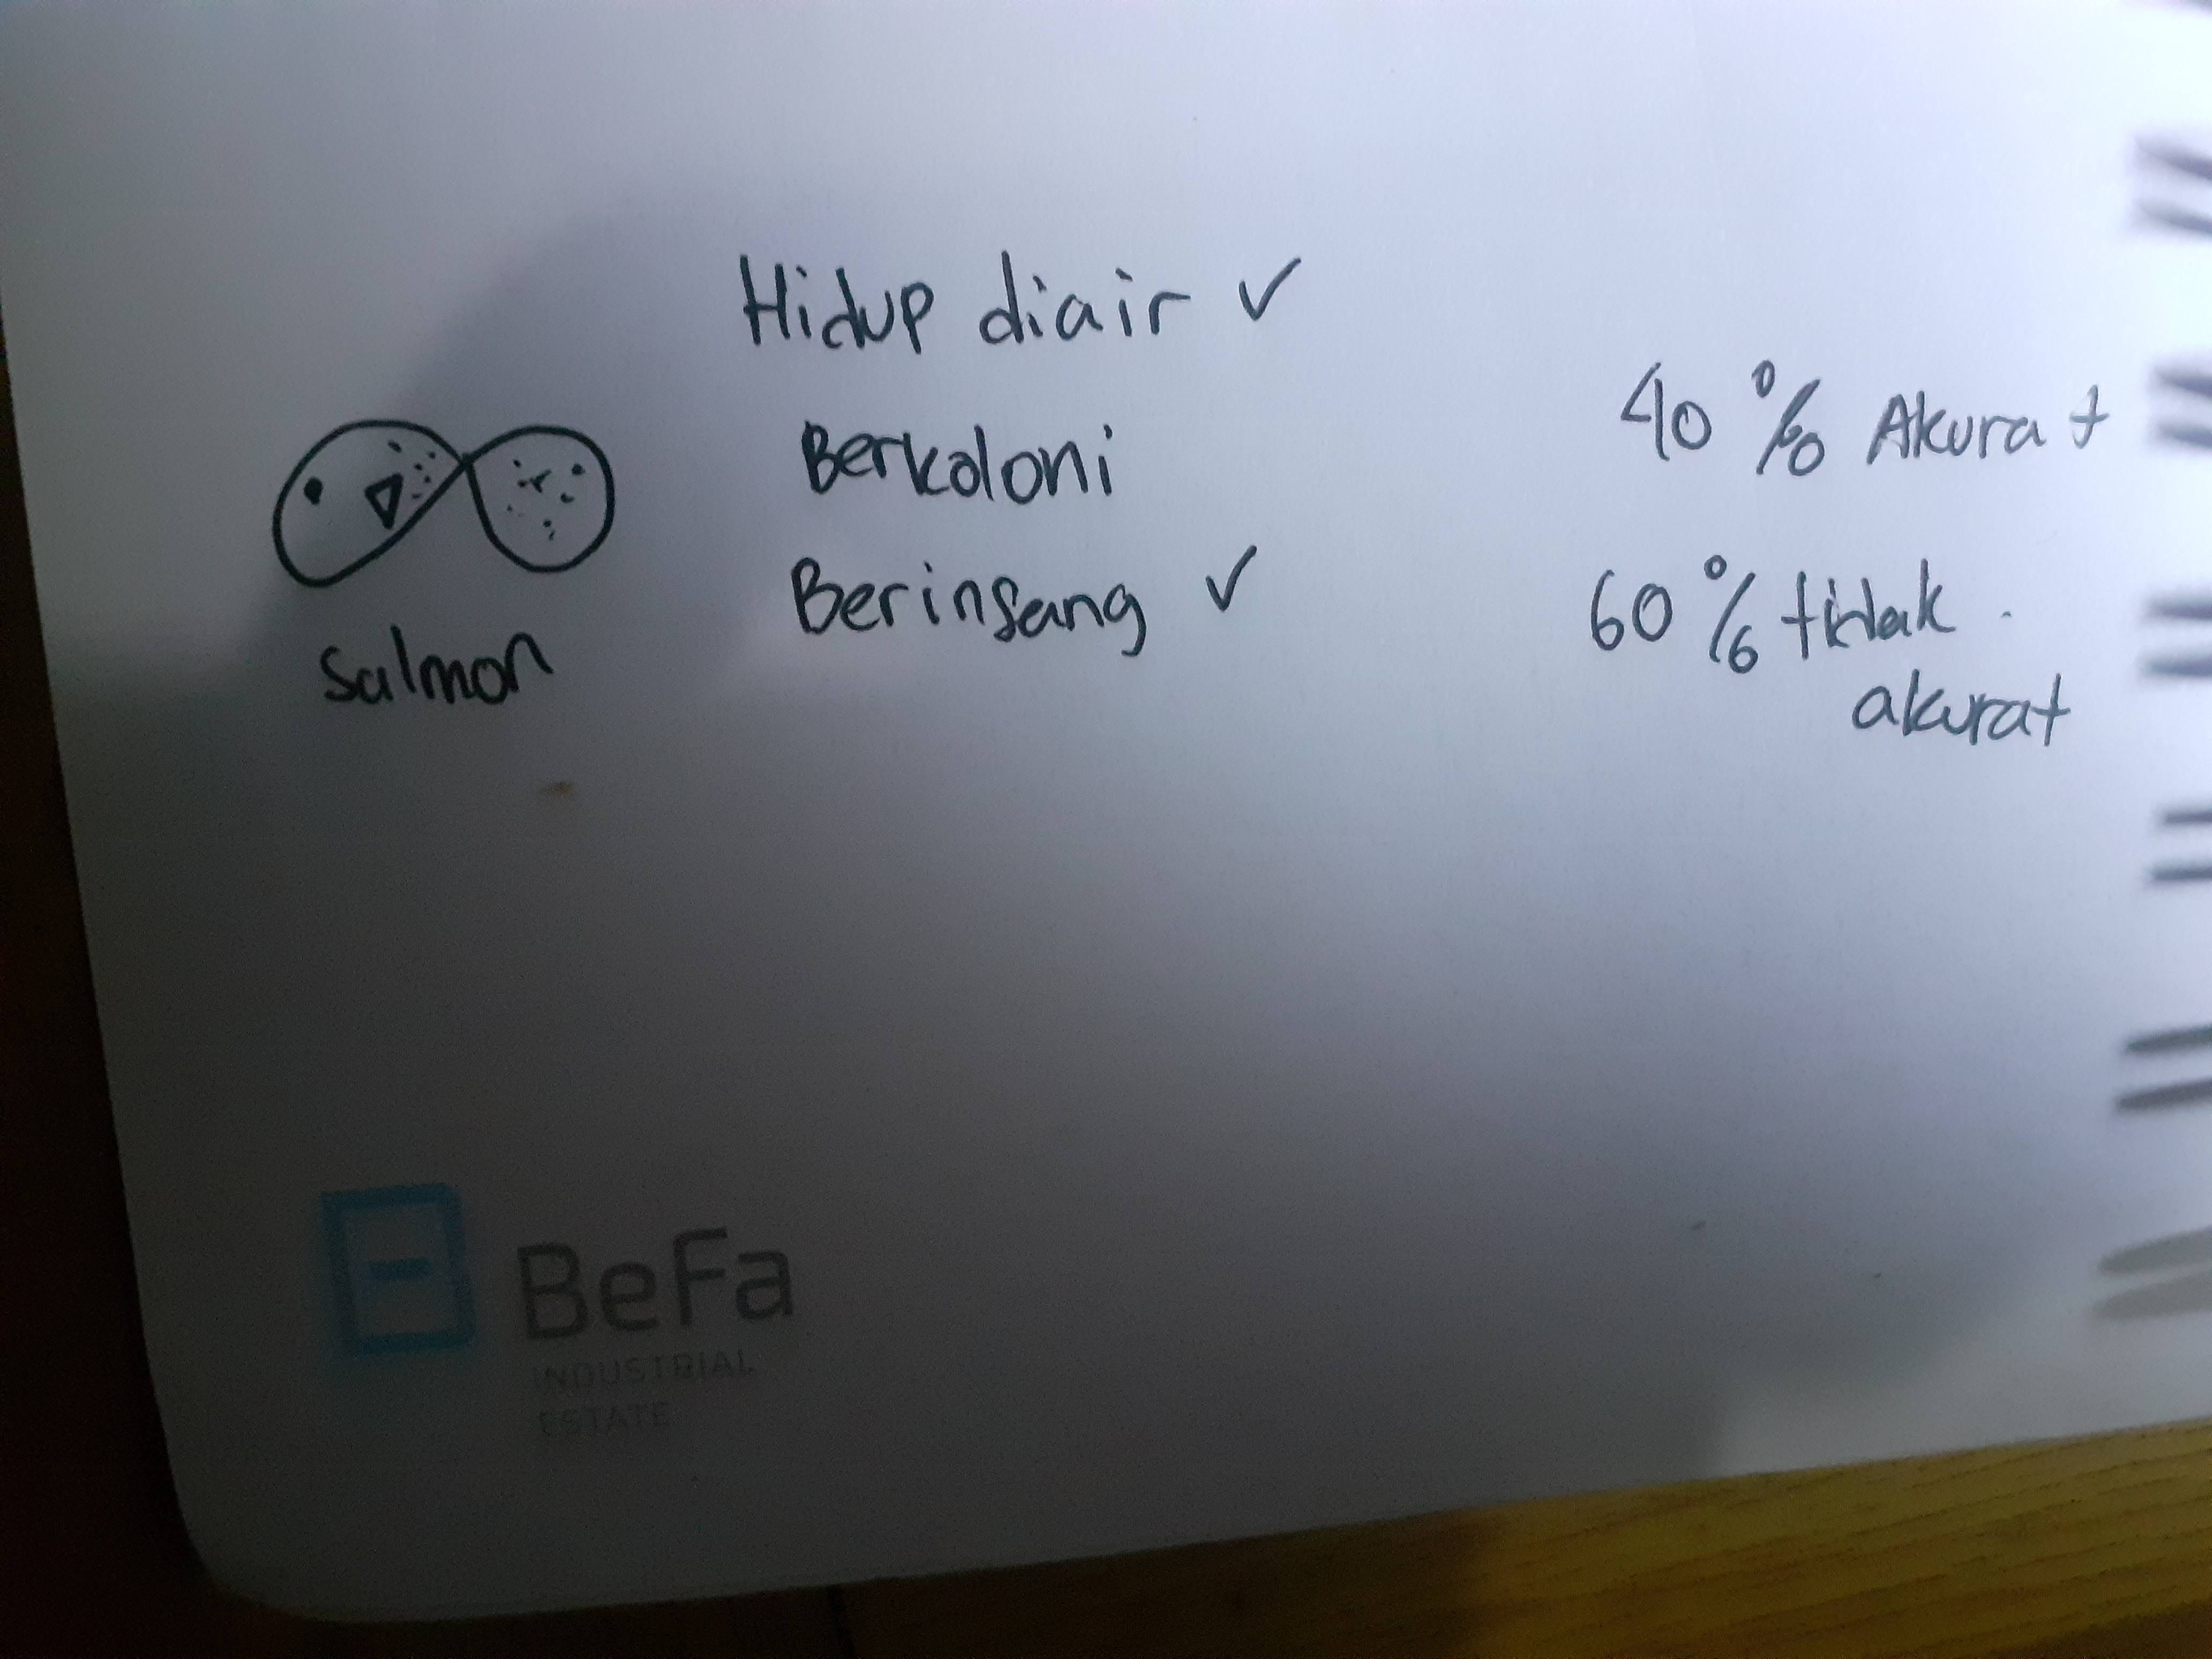
\includegraphics[scale=0.01]{figures/1174043/chapter2/9.jpg}
			\caption{contoh information gain}
			\label{contoh}
		\end{figure}
	\end{enumerate}
		
	\subsection{Scikit-Learn}
	\begin{enumerate}
		\item \hfill \break \lstinputlisting[firstline=8, lastline=11]{src/1174043/chapter2/1.py}
		\begin{figure}[H]
			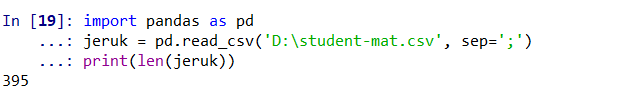
\includegraphics[width=4cm]{figures/1174043/chapter2/hasil1.png}
			\centering
			\caption{Hasil Percobaan 1}
		\end{figure}
		
		\item \hfill \break \lstinputlisting[firstline=15, lastline=18]{src/1174043/chapter2/1.py}
		\begin{figure}[H]
			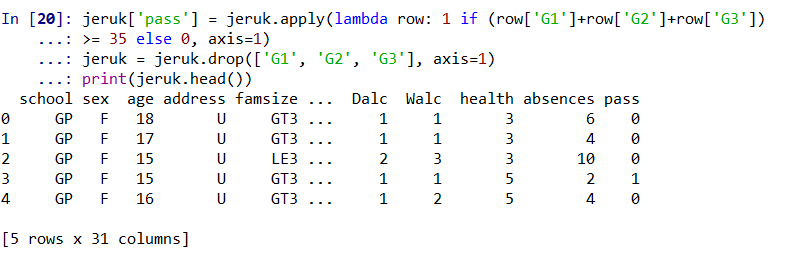
\includegraphics[width=4cm]{figures/1174043/chapter2/hasil2.png}
			\centering
			\caption{Hasil Percobaan 2}
		\end{figure}
		
		\item \hfill \break \lstinputlisting[firstline=22, lastline=23]{src/1174043/chapter2/1.py}
		\begin{figure}[H]
			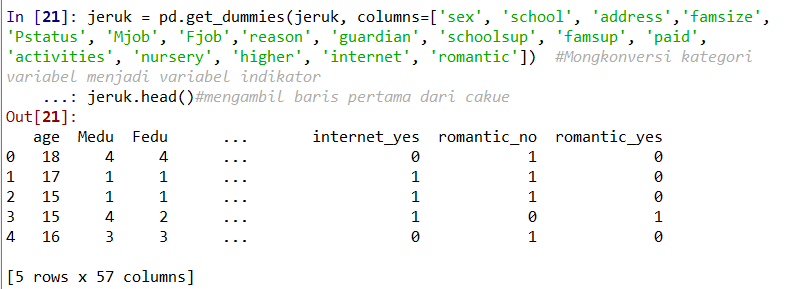
\includegraphics[width=4cm]{figures/1174043/chapter2/hasil3.png}
			\centering
			\caption{Hasil Percobaan 3}
		\end{figure}
		
		\item \hfill \break \lstinputlisting[firstline=28, lastline=40]{src/1174043/chapter2/1.py}
		\begin{figure}[H]
			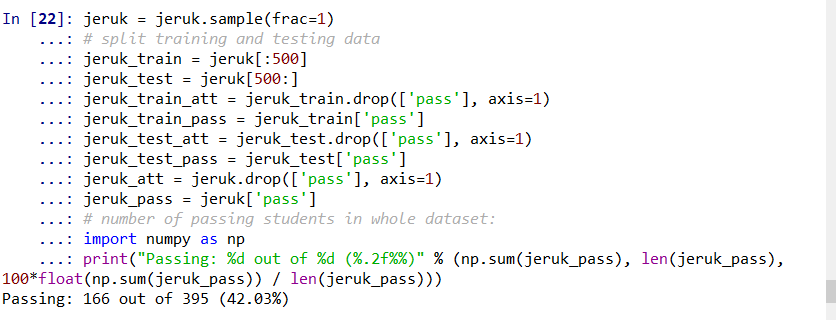
\includegraphics[width=4cm]{figures/1174043/chapter2/hasil4.png}
			\centering
			\caption{Hasil Percobaan 4}
		\end{figure}
		
		\item \hfill \break \lstinputlisting[firstline=45, lastline=47]{src/1174043/chapter2/1.py}
		\begin{figure}[H]
			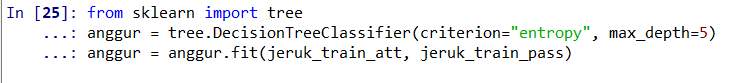
\includegraphics[width=4cm]{figures/1174043/chapter2/hasil5.png}
			\centering
			\caption{Hasil Percobaan 5}
		\end{figure}
		
		\item \hfill \break \lstinputlisting[firstline=52, lastline=57]{src/1174043/chapter2/1.py}
		
		\item \hfill \break \lstinputlisting[firstline=62, lastline=63]{src/1174043/chapter2/1.py}
		\begin{figure}[H]
			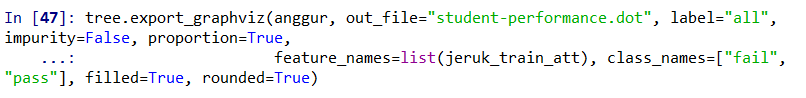
\includegraphics[width=4cm]{figures/1174043/chapter2/hasil7.png}
			\centering
			\caption{Hasil Percobaan 7}
		\end{figure}
		
		\item \hfill \break \lstinputlisting[firstline=67, lastline=67]{src/1174043/chapter2/1.py}
		
		\item \hfill \break \lstinputlisting[firstline=71, lastline=75]{src/1174043/chapter2/1.py}
		\begin{figure}[H]
			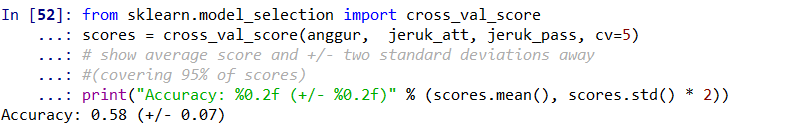
\includegraphics[width=4cm]{figures/1174043/chapter2/hasil9.png}
			\centering
			\caption{Hasil Percobaan 9}
		\end{figure}
		
		\item \hfill \break \lstinputlisting[firstline=79, lastline=83]{src/1174043/chapter2/1.py}
		\begin{figure}[H]
			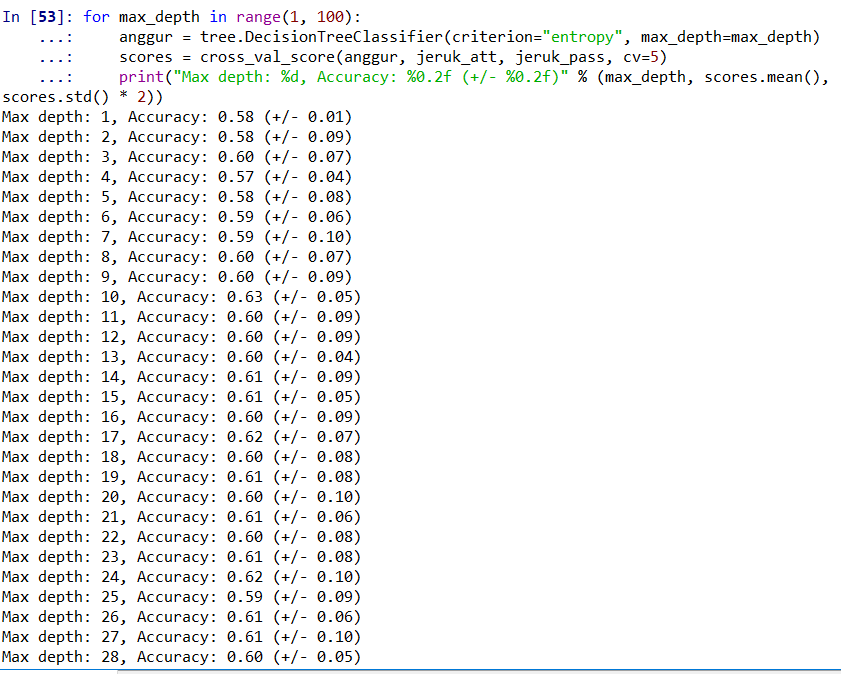
\includegraphics[width=4cm]{figures/1174043/chapter2/hasil10.png}
			\centering
			\caption{Hasil Percobaan 10}
		\end{figure}
		
		\item \hfill \break \lstinputlisting[firstline=86, lastline=96]{src/1174043/chapter2/1.py}
		\begin{figure}[H]
			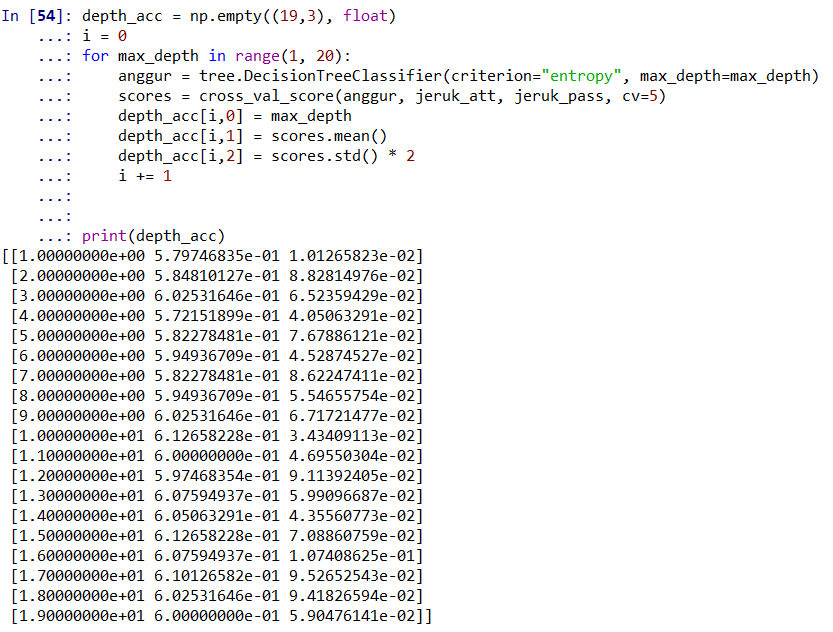
\includegraphics[width=4cm]{figures/1174043/chapter2/hasil11.png}
			\centering
			\caption{Hasil Percobaan 11}
		\end{figure}
		
		\item \hfill \break \lstinputlisting[firstline=100, lastline=103]{src/1174043/chapter2/1.py}
		\begin{figure}[H]
			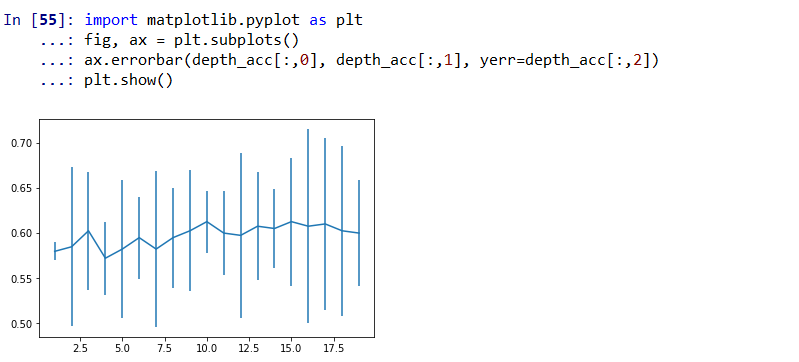
\includegraphics[width=4cm]{figures/1174043/chapter2/hasil12.png}
			\centering
			\caption{Hasil Percobaan 12}
		\end{figure}
	\end{enumerate}